\documentclass{scrbook}

\KOMAoptions{%
    fontsize=10pt,          % Tamaño de fuente
    paper=a4,               % Tamaño del papel
    headings=normal,        % Tamaño de letra para los títulos: small, normal,
                            % big
    parskip=full,           % Espacio entre párrafos: full (una línea) o half
                            % (media línea)
    headsepline=false,      % Una linea separa la cabecera del texto
    cleardoublepage=empty,  % No imprime cabecera ni pie en páginas en blanco 
    chapterprefix=false,    % No antepone el texto "Capítulo" antes del número
    appendixprefix=false,	% No antepone el texto "Apéndice" antes de la letra
    listof=totoc,		    % Añade a la tabla de contenidos la lista de tablas 
                            % y figuras
    index=totoc,			% Añade a la talba de contenidos una entrada para 
                            % el índice
    bibliography=totoc,	    % Añade a la tabla de contenidos una entrada para
                            % bibliografía
    BCOR=5mm,               % Reserva margen interior para la encuadernación. 
                            % El valor dependerá el tipo de encuadernado y del
                            % grosor del libro.
    DIV=10,                 % Cálcula el diseño de página según ciertos 
                            % parámetros. Al aumentar el número aumentamos el
                            % ancho de texto y disminuimos el ancho del margen.
                            % Una opción de 14 producirá márgenes estrechos y
                            % texto ancho.
}

% Set input encoding.
\usepackage[utf8]{inputenc}

% Establish Spanish as the default language. English is also used in the
% abstract.
%   es-tabla - Change "Cuadro" for "Tabla".
\usepackage[english, spanish, es-tabla]{babel}

% Set graphics folder path.
\usepackage{graphicx}
\graphicspath{{images/}}

% Enable graphics placement.
\usepackage{float}

% Apply color to tables.
\usepackage{colortbl}

% Set title page background image.
\usepackage{eso-pic}
\newcommand\BackgroundPic{%
	\put(0,0){%
		\parbox[b][\paperheight]{\paperwidth}{%
			\vfill
			\centering
			
\includegraphics[width=\paperwidth,height=\paperheight,%
			keepaspectratio]{ugr/portada-sencilla-color}%
			\vfill
}}}

% Add the euro symbol.
\usepackage{marvosym}
\DeclareUnicodeCharacter{20AC}{\EUR{}}

% Code listings.
\usepackage{listings}

\usepackage{hyperref}
\usepackage{booktabs}
\usepackage{bookmark}

% Change second level label item to a dash.
\renewcommand{\labelitemii}{--}

\begin{document}

\frontmatter
\begin{titlepage}
    \AddToShipoutPicture*{\BackgroundPic}

    \begin{addmargin}[2.575cm]{0cm}
        \begin{flushleft}
            \Large
            \hfill\vfil

            \large{\textsf{Escuela Técnica Superior en Ingenierías Informática y de Telecomunicación}}
            \vfill

            {\large\textsc{Máster Universitario en Ingeniería Informática}} \vfill


            {\large\textsc{trabajo de fin de máster}}

            \begingroup
            \Huge{Título del TFM}
            \endgroup

            \vfill\vfill\vfill\vfill

            \textsf{\normalsize{Presentado por:}}\\
            {\normalsize\textrm{Víctor Vázquez Rodríguez}}
            \bigskip

            \textsf{\normalsize{Tutor:}}\\
            {\normalsize\rmfamily{
                Antonio Javier Díaz Alonso\\
                \emph{Departamento de Arquitectura y Tecnología de Computadores}
            }}

            \bigskip
            \textsf{\normalsize{Curso académico 2020-2021}}
        \end{flushleft}
    \end{addmargin}
\end{titlepage}
\cleardoublepage
\pdfbookmark[1]{Agradecimientos}{Agradecimientos}

\chapter*{Agradecimientos}

Al Dr. Antonio Javier Díaz Alonso, tutor de este trabajo, por guiarme y
aportarme su experiencia académica.

A mis padres, por darme la oportunidad de estudiar y seguir mi propio camino.

Al Dr. Juan Antonio Vázquez Rodríguez, mi hermano, por ser mi referente de
esfuerzo, trabajo, bondad y humildad.

A mi novia, Rosa, por creer siempre en mí y estar a mi lado pase lo que pase.

A mis compañeros de promoción del Máster, por hacerme sentir como en casa lejos
de ella.

\cleardoublepage
\pdfbookmark[1]{Resumen}{Resumen}

\chapter*{Resumen}

\selectlanguage{spanish}
Con el advenimiento de la Industria 4.0, las empresas buscan incorporar técnicas
de inteligencia artificial y análisis de datos a sus instalaciones y procesos
industriales con el objetivo de mejorar la productividad y la autonomía. En este
trabajo, se plantea la posibilidad de usar tecnologías de contenerización de
procesos para el despliegue eficiente de estas nuevas tareas junto con las de
tiempo real habituales en los sistemas de control industrial, estudiando las
distintas tecnologías posibles y realizando un análisis del rendimiento de
tareas de tiempo real contenerizadas con Docker. Además, se diseña e implementa
una herramienta software que sirve como prueba de concepto para el despliegue y
la orquestación de este tipo de tareas sobre entornos distribuidos mediante el
uso de contenedores.

\selectlanguage{english}
\itshape
As Industry 4.0 gets closer, companies are looking to incorporate artificial
intelligence and data analysis techniques to their facilities and industrial
processes with the objective of improving productivity and autonomy. This paper
proposes the use of processes containerization techonologies for efficient
deployment of these new tasks along with the real-time tasks that are common in
industrial control systems, studying different possible techonologies and
analysing the performance of real-time tasks containerized using Docker.
Finally, a proof-of-concept software tool for deployment and orchestration of
this type of tasks on distributed environments by means of containers.

\selectlanguage{spanish}

\cleardoublepage
\pdfbookmark[1]{\contentsname}{toc}

\tableofcontents
\listoffigures
\listoftables
\lstlistoflistings

\cleardoublepage

\mainmatter
\chapter{Introducción}

\section{Motivación y contexto}

El Programma 101 es considerado por muchos como el primer ordenador de uso
personal. Producido por la empresa italiana Olivetti entre los años 1962 y 1964,
este dispositivos seasimilaba más a una calculadora que al concepto de ordenador
que se tiene en la actualidad. Casi 60 años después, los ordenadores han
evolucionado hasta convertirse en un objeto asequible y casi indispensable,
teniendo la mayor parte de la sociedad acceso a algún dispositivo con capacidad
de computación. Aspectos de nuestra vida como el ocio, serían muy diferentes sin
las redes sociales o los servicios online. Esta evolución de los ordenadores y
la computación en general continúa hoy en día, buscando conectar dispositivos
cotidianos a internet e incorporar en ellos cierta capacidad de procesamiento.
Televisores inteligentes en los que instalar aplicaciones, robots aspiradores
que funcionan de manera autónoma, frigoríficos que permiten ver el estado de los
alimentos que almacenan, todos estos productos surgen de la expansión de los
ordenadores hasta todos los rincones de nuestras vidas, con el objetivo final de
hacerla más sencilla para los humanos. Esta expansión no está ocurriendo solo en
los hogares, si no que se avanza hacia un mundo más conectado donde
aparentemente todo lo que nos rodea tenga acceso a la red.

La industria no es ajena a este cambio, ya que la aplicación del internet de las
cosas (IoT por sus siglas en inglés) a los procesos industriales podría aportar
beneficios muy importantes como son el aumento de la productividad, de la
calidad de los productos o de la seguridad de las instalaciones. No obstante, se
trata de un proceso de implantación complejo y de muy largo plazo, debido a los
estrictos requisitos de algunos sectores industriales. Las fábricas y plantas de
producción relegan las tareas de control de sus operaciones a los sistemas de
control industriales o ICSs (\textit{Industrial Control Systems}). Normalmente,
estos sistemas deben responder ante eventos que ocurren en las instalaciones en
ventanas de tiempo muy pequeñas, dependiendo del proceso concreto y sus riesgos
asociados. La fiabilidad de estos sistemas y su tolerancia ante los fallos es de
gran importancia, siendo crucial la verificación de estos aspectos durante su
diseño y desarrollo. Es por estos requisitos tan estrictos que, en muchos casos,
para la implantación de los ICSs se utilizan tanto \textit{hardware} como
\textit{software} específicos y que ya han sido validados para este tipo de
aplicaciones. No obstante, el uso de estas herramientas también plantea algunos
inconvenientes, como por ejemplo la difícil interoperabilidad con otros sistemas
debido a la naturaleza cerrada de las mismas o la reutilización del código en
otras plataformas, lo que acorta la vida útil del \textit{software}.

Desde esta situación se afronta el avance hacia la cuarta revolución industrial
o Industria 4.0. Uno de los objetivos principales que se persigue es la
automatización completa de los procesos industriales, haciando que sean
independientes y autogestionados, aumentando así su eficiencia, productividad y
seguridad. Para conseguir este objetivo, es necesario incorporar a estos
procesos las nuevas técnicas de aprendizaje automático y análisis de grandes
volúmenes de datos, construyendo sistemas experots capaces de tomar decisiones
propias para su funcionamiento y gestión (p. ej., modificar el ritmo de
producción en base a predicciones sobre la demanda). Aunque estos sistemas
expertos se podrían desplegar en plataformas separadas de las que habitan los
ICSs, esto duplica los costes de infraestructura y hace también más difícil el
mantenimiento de la misma. Por ello, hay una tendencia cada vez mayor hacia la
ejecución de tareas con distintos niveles de criticalidad en una misma
plataforma. Por otra parte, las tareas de aprendizaje máquina suelen requerir de
una capacidad de computación relativamente elevada, sobre todo cuando la
cantidad de datos sobre la que se trabaja es grande. Un solo dispositivo no
sería capaz de gestionar estas tareas de forma eficiente si, además, debe
realizar tareas críticas de control, dificultando también que pueda cumplir con
sus requisitos en ese aspecto. Aparecen entonces nuevos paradigmas de
computación, como el \textit{fog} o el \textit{edge computing}, que pretenden
decentralizar el procesamiento, alejándolo de la nube y llevándolo a elementos
intermedios más cercanos a las fuentes de datos o a los dispositivos del borde
de la red, respectivamente. En estos paradigmas, se persigue la máxima
utilización de la capacidad de computación de los dispositivos presentes en la
red, distribuyendo entre ellos las tareas necesarias de forma dinámica.

Dentro de este campo, se están llevando a cabo muchas investigaciones para
validar la efectividad de estos nuevos modelos y hacerlos realidad, además de
comprobar su efectividad en el ámbito industrial. Uno de los planteamientos más
prometedores es el que conlleva la aplicación de tecnologías de virtualización a
los sistemas de control industrial, permitiendo su despliegue y ejecución
distribuida en convivencia con otros procesos. Estas tecnologías, que han
sufrido un desarrollo masico en los últimos años debido al auge de la
computación en la nube, pueden ahora ser claves para asegurar la resiliencia y
robustez de los ICSs en entornos distribuidos.

Por todo esto, este trabajo abordará la complejidad de los problemas descritos
intentando buscar mecanismos que simplifiquen la gestión de los sistemas
\textit{fog}/\textit{edge}. Partiremos de la experiencia previa en trabajos con
contenedores orientados al análisis de sus prestaciones para la ejecución de
tareas con restricciones temporales, responsables de las ideas aquí propuestas y
base fundamental de parte de la motivación de este trabajo. Además, esta línea
de investigación tiene mucho potencial para mejorar los sistemas de control
implementados en la actualidad, permitiendo por tanto una contribución
importante tanto en aspectos industriales como científicos, lo que aumenta aún
más nuestro interés en esta temática.

\section{Objetivos}

De cara a la realización de este trabajo, se han planteado los siguientes
objetivos a cumplir:

\begin{itemize}
    \item Comprender los conceptos básicos sobre sistemas operativos de tiempo
          real, algoritmos de planificación y sistemas de control industriales.
    \item Analizar las soluciones de tiempo real basadas en GNU/Linux existentes.
    \item Estudiar la viabilidad y rendimiento de las tecnologías de
          contenerización para la ejecución de tareas con restricciones temporales.
    \item Diseñar e implementar una herramienta de despliegue de tareas de
          tiempo real mediante contenedores que sirva como prueba de concepto.
    \item Caracterizar las prestaciones de la herramienta desarrollada,
          identificando posibles aplicaciones y/o mejoras de la misma.
\end{itemize}

Una parte relevante de los objetivos del presente proyecto están asociados al
estudio y caracterización de tecnologías, así como al análisis del mercado, que
se justifica por un enfoque innovador orientado al desarrollo de sistemas para
\textit{fog computing}. Esto, junto con los conocimientos adquiridos sobre
implementación de sistemas de tiempo real, será clave para que la herramienta
desarrollada como prueba de concepto sea lo más eficiente y funcional posible.

Por otra parte, en los objetivos también se hace hincapié en el uso de
soluciones basadas en GNU/Linux, como parte de un fuerte compromiso con las
herramientas libres y de código abierto. Algunos de los sistemas operativos de
tiempo real más conocidos y usados son de código propietario y es necesario
adquirir licencias para utilizarlos, lo cual no favorece ni el aprendizaje ni la
reutilización del software desarrollado para estas plataformas. Últimamente, se
han realizado contribuciones importantes al kernel de Linux para mejorar el
soporte que ofrece a cargas de trabajo de este tipo, además de los múltiples
proyectos más especializados que está llevando a cabo la comunidad. En esta
aproximación, hemos considerado primordial la extensión del software libre,
apoyando su uso siempre que sea posible. Por ello, la herramienta planteada se
diseñará en torno al despliegue de tareas en sistemas GNU/Linux.

\section{Planificación}

\section{Material y métodos}

En esta sección, se presentan todas las herramientas que se han usado para
llevar a cabo este proyecto, además de las metodologías de trabajo seguidas. En
la figura \ref{fig:01-tools} se puede ver una recopilación de los logotipos de
todas estas herramientas, las cuales se van a exponer en detalle a continuación.

En un proyecto de desarrollo de código como es este, una de las herramientas más
importantes es la de control de versiones. En nuestro caso, se ha usado
\textbf{Git} debido a que es una herramienta de código libre y, además, es la
más conocida y usada. El repositorio remoto se ha alojado en \textbf{GitHub}, la
popular plataforma de desarrollo de código colaborativo. El desarrollo de código
como tal se ha hecho con \textbf{Visual Studio Code}, un editor de texto de
Microsoft que, aunque ofrece menos funcionalidad de serie que los entornos de
desarrollo (IDEs) especializados, también es mucho más liviano y rápido. Además,
esta funcionalidad se puede extender enormemente mediante extensiones, pudiendo
convertirlo casi en un IDE adaptado a las necesidades concretas del usuario.
Gracias a estas extensiones, se puede usar el mismo editor para distintos
programar en distintos lenguajes, lo cual ha sido una de las principales razones
por las que se ha escogido.

Como ya se ha indicado en la sección anterior, se ha aplicado un SCRUM adaptado
como metodología de planificación, gestión y seguimiento del proyecto, usando un
tablero Kanban para la visualización de las tareas. Concretamente, se ha usado
el tablero que ofrece GitHub como parte de sus herramientas para la gestión de
proyectos. Las tareas se añaden a los repositorios como \textit{issues}, los
cuales se añaden al tablero para controlar su estado de realización. El
beneficio que nos aporta el uso de GitHub para esto es el de tener una
plataforma unificada tanto para la gestión del proyecto como para su desarrollo.
Esta integración permite flujos de trabajo muy interesantes, como por ejemplo
referenciar los \textit{issues} ya mencionados en los mensajes de
\textit{commit}, de forma que se vinculan los cambios realizados con la tarea en
la que se engloban. La gestión del proyecto es, por tanto, más directa y
sencilla.

\textbf{Incorporar imagen del tablero del proyecto de GitHub}

Los diagramas que se presentan a lo largo de este trabajo, incluidos los que
componen el diseño de la herramienta desarrollada y sus componentes, se han
creado con la herramienta online \textbf{draw.io}. Al integrarse directamente
con Google Drive, se puede usar desde el navegador, siendo una solución muy
cómoda y accesible para la creación de estos diagramas.

En cuanto al desarrollo y despliegue de la herramienta planteada, se han
utilizado varias tecnologías. Los lenguajes de programación son Python y C, muy
conocidos y utilizados en la industria. C es el lenguaje de referencia para la
programación de sistemas y las tareas de bajo nivel, mientras que Python ofrece
una sintaxis muy sencilla para la implementación de herramientas como
aplicaciones o servidores. Python también posee una nutrida colección de
librerías para distintos casos de uso, lo cual también fue muy atractivo para su
elección. En este proyecto, se usan varias de estas librerías para facilitar la
implementación de algunos aspectos de la herramienta. Destacamos las siguientes:

\begin{itemize}
    \item \textbf{hug} - Escritura de APIs sencilla y sin ataduras. Esta
          librería trata de competir con otras más conocidas como Flask, proponiendo
          un modelo mucho más simple y dando más libertad al desarrollador.
    \item \textbf{click} - Más que una librería, se trata de un
          \textit{framework} para la implementación de aplicaciones de línea de
          comandos (CLI). Ofrece todas las utilidades que se pueden necesitar para
          este tipo de aplicaciones, como es la generación automática de páginas de
          ayuda.
    \item \textbf{marshmallow} - Esta librería permite la sencilla
          deserialización y serialización de objetos JSON a objetos Python. Esto es
          especialmente útil al trabajar con servicios web, ya que se pueden leer los
          datos JSON recibidos y validarlos frente a un esquema de datos definido por
          el desarrollador.
    \item \textbf{pymongo} - Ejecución de consultas sobre bases de datos
          MongoDB, que son las usadas en este proyecto.
    \item \textbf{paramiko} - Herramientas para trabajar con SSH desde Python.
          Esencial para el despliegue de las tareas sobre los nodos.
    \item \textbf{docker} - La librería oficial de Docker para Python. Con ella,
          se puede conectar con un servidor Docker (local o remoto) para ejecutar
          operaciones de construcción de imágenes o lanzamiento de contenedores.
    \item \textbf{requests} - Es la librería más conocida para la realización de
          peticiones HTTP en Python.
    \item \textbf{unittest} - Aunque no se trata de una librería externa como
          las demás, ya que forma parte de la librería estándar de Python, merece ser
          destacada por ser la utilizada para la escritura y ejecución de las pruebas
          del código desarrollado.
\end{itemize}

Además de estas librerías, se han usado otras para el análisis y formateo del
código como son \textbf{pylint} y \textbf{autopep8}.

Como ya se ha mencionado, la herramienta desarrollada trabaja con
\textbf{MongoDB} para la gestión del almacenamiento persistente de los datos y
el acceso a los mismos. Se trata de un gestor de bases de datos documental que
pertenece a la familia NoSQL (\textit{Not only SQL}). Las bases de datos
documentales divergen del modelo relacional tradicional que siguen otros
gestores tan famosos como MySQL o PostgreSQL. No existen los conceptos de tabla
o fila, sino que se almacenan colecciones de documentos no estructurados. En el
caso de MongoDB, se trabaja con documentos JSON, formato ampliamente usado en el
entorno web para la transmisión de datos debido a su legibilidad y velocidad de
serialización/deserialización. Cuando decimos que los documentos son no
estructurados, nos referimos a que no tienen por qué poseer los mismos campos,
ya que no hay un esquema definido a seguir. MongoDB no cumple con ACID, pero es
una pérdida aceptable a cambio de la flexibilidad y facilidad de uso que nos
ofrece. Además, el lenguaje de consultas es mucho más claro e intuitivo que SQL,
permitiendo realizar consultas de envergadura similar.

\begin{figure}[H]
    \centering
    
\includegraphics[width=0.7\textwidth]{01-introduction/tools.png}
    \caption{Logotipos de las herramientas utilizadas. De izquierda a derecha y%
        de arriba a abajo: Python, Docker, Raspberry Pi, GitHub, VS Code y
        draw.io}
    \label{fig:01-tools}
\end{figure}

La idea principal en torno a la cual gira este trabajo es la del uso de
contenedores para el despliegue de tareas de tiempo real. En este sentido,
\textbf{Docker} es la tecnología de contenerización en la que nos hemos apoyado
para la implementación de la herramienta propuesta. Esta elección recae
principalmente en el hecho de que se trata del motor de contenedores más
conocido y utilizado. De la mano de Docker, también se ha utlizado
\textbf{Docker Compose} para el despliegue sencillo de un entorno de desarrollo
completo que permita replicar un despliegue de producción de forma simplificada.
Las imágenes de contenedores definidas en este proyecto, se han alojado en el
repositorio de imágenes \textbf{DockerHub}, aprovechando que proporciona un
sistema de construcción automática de imágenes.

Para realizar las pruebas del sistema desarrollado, se ha usado una
\textbf{Raspberry Pi 4B}, concretamente la que se muestra en la figura
\ref{fig:01-raspberry-pi}. Se trata de un SBC (\textit{Single Board Computer})
de bajo coste y muy versátil, pudiendo usarse para infinidad de aplicaciones.
Las características detalladas de esta plataforma se pueden ver en la tabla \ref{tab:01-raspberry-specs}.

\begin{table}[H]
    \centering
    \begin{tabular}{ |>{\columncolor[gray]{0.8}}l|p{0.5\textwidth}| }
        \hline
        \textbf{Procesador}          & Cortex-A72                \\
        \hline
        \textbf{Arquitectura}        & ARMv7                     \\
        \hline
        \textbf{Número de núcleos}   & 4                         \\
        \hline
        \textbf{Frecuencia de reloj} & 1500 MHz                  \\
        \hline
        \textbf{RAM}                 & 4 GB                      \\
        \hline
        \textbf{Sistema operativo}   & Raspberry Pi OS Lite 4.19 \\
        \hline
    \end{tabular}
    \caption{Especificaciones de la Raspberry Pi usada en el trabajo}
    \label{tab:01-raspberry-specs}
\end{table}

El sistema operativo de este dispositivo es GNU/Linux (concretamente, basado en
Debian), y se le ha aplicado la revisión 24 del parche de tiempo real
\textbf{PREEMPT-RT}. Este parche aporta al sistema la capacidad de realizar
planificación de procesos apropiativa.

\begin{figure}
    \centering
    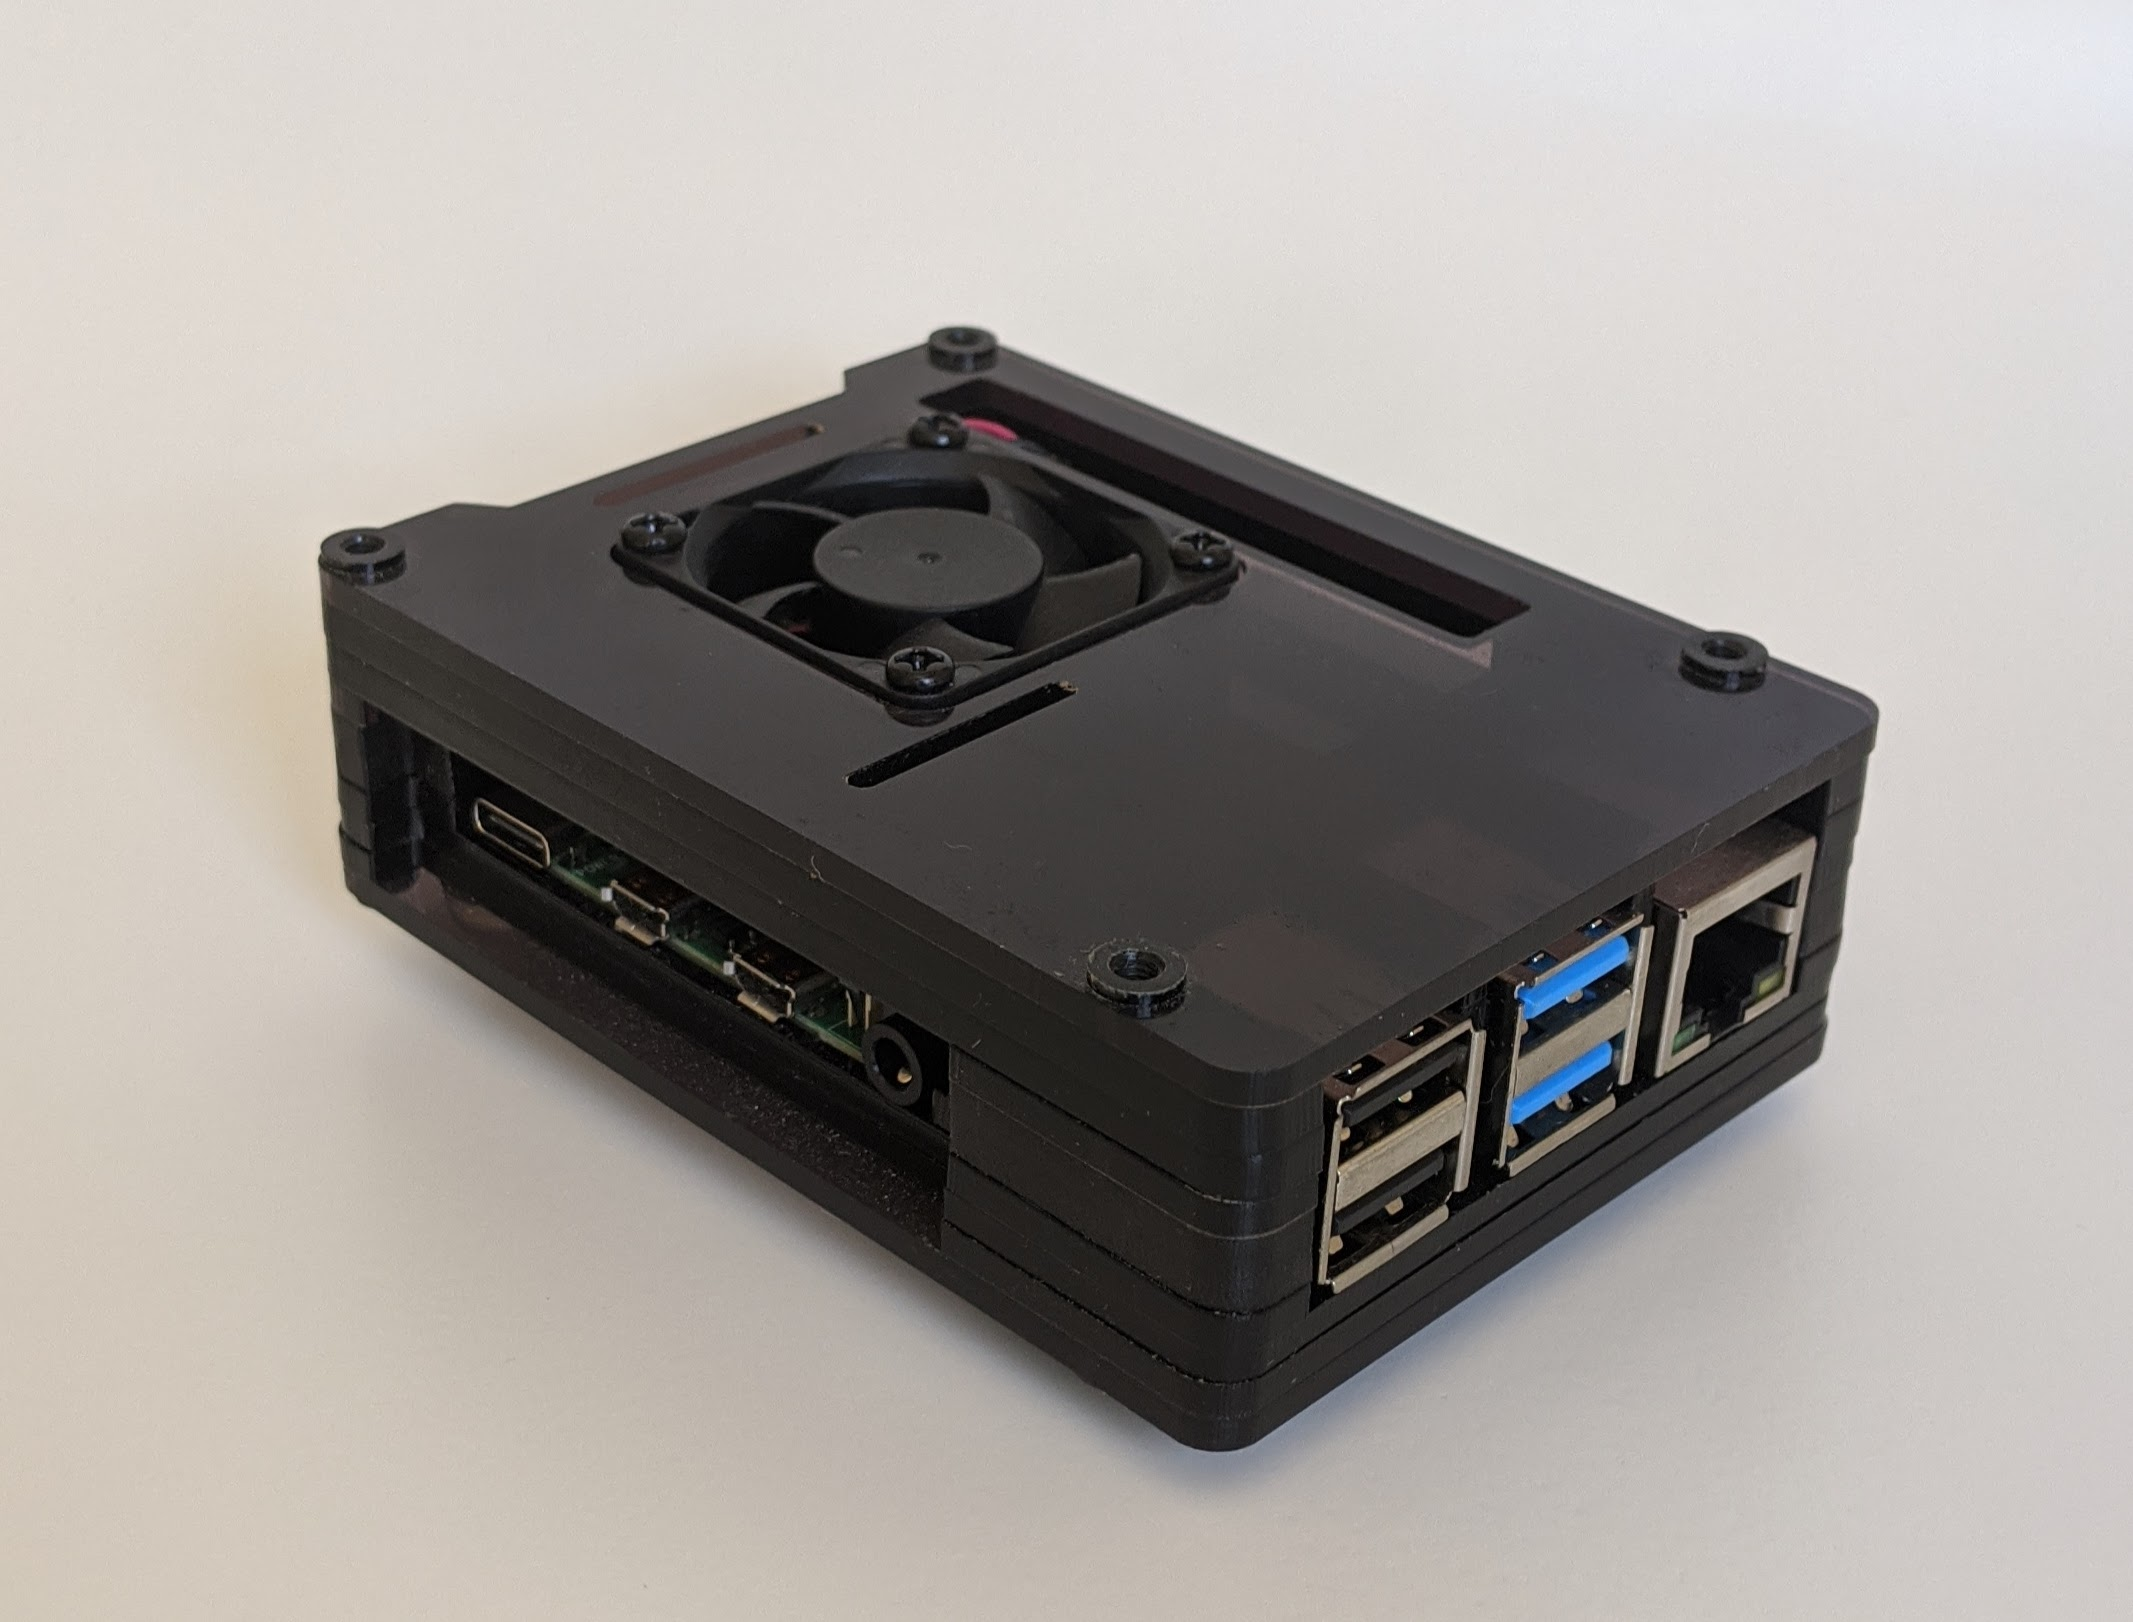
\includegraphics[width=0.8\textwidth]{01-introduction/raspberry-pi.jpg}
    \caption{Raspberry Pi 4B utilizada en el trabajo}
    \label{fig:01-raspberry-pi}
\end{figure}

\section{Estructura de la memoria}

La estructura de la presente memoria es la siguiente:

En el capítulo 1, se ha introducido el proyecto y explicado tanto la motivación
detrás del mismo como los objetivos planteados, la planificación seguida y las
herramientas, tecnologías y metodologías que se han utilizado.

En el capítulo 2, se realiza un estudio en profundidad del estado de la técnica
en lo relativo a los sistemas confiables, las tareas de tiempo real y las
tecnologías de virtualización. Se presentan otros estudios interesantes llevados
a cabo en esta área y se introducen todos los conceptos relevantes.

En la sección 3, se aborda el diseño de una herramienta para el despliegue y
seguimiento de tareas de tiempo real en entornos distribuidos, así como su
implementación y prueba. Se presentan los resultados obtenidos y se discute
sobre los mismos.

En la sección 4, se realiza una revisión del proyecto completo y se presentan
las conclusiones, así como las maneras en las que se puede extender y mejorar el
trabajo realizado.

\chapter{Revisión del estado de la técnica}

Antes de poder aventurarnos el desarrollo de una herramienta para la
orquestación de tareas de tiempo real usando contenedores, es necesario
estudiar y comprender los fundamentos y peculiaridades de diversos campos como
son los sistemas de tiempo real, la planificación de procesos, la computación en
la nube o las tecnologías de virtualización. En este capítulo, se introducen los
conceptos más importantes de estos campos, además de revisar otros trabajos
realizados con el objetivo de comprobar cuál es el estado de la investigación
en dichos temas.

\section{Sistemas empotrados, confiables y de criticalidad mixta}

Los ordenadores y teléfonos inteligentes que usamos a diario nos permiten
realizar multitud de tareas diferentes: desde leer el correo o navegar por
internet hasta editar imágenes y vídeos o realizar videollamadas. Aunque no nos
demos cuenta, interactuamos habitualmente con muchos más sistemas informáticos
además de los ya mencionados. La computación está presente en los coches, los
trenes, los aviones, los satélites espaciales, los televisores o las lavadoras.
Estos sistemas, que reciben el nombre de sistemas empotrados, son diseñados para
llevar a cabo de manera óptima un conjunto de tareas específico, frente al
enfoque generalista de los ordenadores de uso personal. Como se introduce en
\cite{wolf_high-performance_2014}, los sistemas empotrados son comunes en
contextos en los que el rendimiento es primordial, como son las comunicaciones
de red o la compresión/decompresión de audio y vídeo para retransmisiones en
directo. En este libro se exponen diversas aplicaciones de los sistemas
empotrados de alto rendimiento para sistemas ciber-físicos o CPS
(\textit{Cyber-Physical Systems}). Los CPS son, en esencia, sistemas
informáticos que interactúan con procesos físicos, actuando en función de los
cambios en su entorno. Este aspecto hace que el diseño y la implementación de
los CPS difiera considerablemente del resto de sistemas empotrados, ya que hay
que prestar especial atención a las características del entorno en el que se
desplegará el sistema y a los mecanismos de entrada y salida (interacción con el
entorno), además de optimizar el consumo de memoria y procesamiento para cumplir
con las limitaciones del hardware \cite{lee_introduction_2016}.

En algunos casos, estos sistemas son críticos, lo que significa que un fallo en
su funcionamiento supone daños graves a las personas o al medio ambiente. Este
es el caso de los aviones, los trenes o las plantas nucleares, por ejemplo. En
estos sistemas, cobra especial importancia el concepto de confiabilidad, es
decir, garantizar el correcto funcionamiento del sistema en todo momento. En la
figura \ref{fig:01-dependability} se pueden apreciar los atributos que debe
poseer un sistema confiable. A nivel de software, existen arquitecturas y
patrones de diseño orientados a garantizar la tolerancia ante los fallos del
mismo \cite{pullum_software_2001}\cite{randell_system_1975}. Por otra parte, la
replicación de componentes \cite{hutchison_dependable_2006} es una técnica muy
usada tanto para el software como el hardware. Lo que se intenta con la
replicación es asegurar que un cálculo o procesamiento se lleva a cabo de forma
correcta, aunque alguna de las réplicas falle. En \cite{amin_review_2019}, se
realiza una revisión de los sistemas de control tolerantes ante fallos
dividiéndolos en tres tipos: AFTCS (\textit{Active Fault Tolerant Control
  Systems}), PFTCS (\textit{Passive Fault Tolerant Control Systems}) o HFTCS
(\textit{Hybrid Fault Tolerant Control Systems}). Para cada uno de estos tipos,
los autores presentan las principales arquitecturas usadas, los modelos de
análisis matemático usados para su validación y las últimas técnicas usadas para
su diseño. Por otra parte, el estudio realizado en \cite{shan_survey_2019} tiene
como objetivo analizar la aplicación de los estándares de seguridad, protección
y privacidad al diseño y desarrollo de sistemas confiables, llegando los autores
a la conclusión de que cada vez están ganando más popularidad los de protección
y privacidad, aunque los procesos para asegurar estos aspectos son menos maduros
que los relacionados con la seguridad. Además, también se identifica una falta
de acción combinada en estos aspectos, trabajando normalmente por separado en
cada uno de ellos.

\begin{figure}
  \centering
  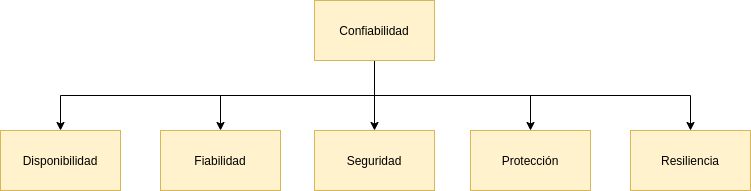
\includegraphics[width=\textwidth]{01-introduction/dependability.png}
  \caption{Principales aspectos de la confiabilidad}
  \label{fig:01-dependability}
\end{figure}

Para muchos sistemas de control, el tiempo es también un aspecto relevante a la
hora de garantizar su correcto funcionamiento. Estos son los llamados sistemas
de tiempo real. En un sistema normal, en el que se obtiene una salida al aplicar
una cierta lógica sobre la entrada, la corrección de dicha salida depende de la
corrección de la lógica aplicada, es decir, del cálculo realizado. No obstante,
cuando hablamos de sistemas de tiempo real, la corrección de la lógica no es
suficiente para determinar que el funcionamiento es correcto, sino que esta
corrección depende también del momento temporal en el que se obtiene
\cite{gambier_real-time_2004}. En otras palabras, si el cálculo es correcto pero
el resultado no llega en el momento en el que se necesita, se considera como un
fallo del sistema. Las tareas que ejecuta un sistema de tiempo real están, por
tanto, sujetas a restricciones temporales. Normalmente, hablamos de un tiempo
límite o \textit{deadline} antes del cuál se debe haber completado la tarea.
Comúnmente, se suelen clasificar las tareas en dos tipos dependiendo de las
consecuencias de incumplir con sus restricciones temporales:

\begin{itemize}
  \item Tareas de tiempo real «blandas»: Se denominan así aquellas tareas en las
        que no completar las mismas antes del límite supone una reducción en la
        calidad del servicio (QoS).
  \item Tareas de tiempo real «duras»: En estas tareas, el no cumplir con las
        restricciones temporales supone un fallo grave del sistema con posibles
        consecuencias catastróficas.
\end{itemize}

Para implementar estos sistemas, se hace uso de herramientas y algoritmos de
planificación de procesos específicos que permiten la ejecución de estos tipos
de tareas cumpliendo con sus restricciones temporales. Esto se explica en más
detalle en la sección \ref{sec:real-time}.

En este trabajo, nos centraremos especialmente en los sistemas de control
aplicados a entornos industriales. Debemos diferenciar entre dos conceptos: PCS
(\textit{Process Control System}), que es el sistema encargado de controlar una
parte concreta de la planta (p. ej., una turbina o un brazo robótico), e ICS
(\textit{Industrial Control System}), que se refiere al control de toda la
planta al completo. Un ICS está compuesto, por tanto, de múltiples PCS que se
encargan de controlar los distintos aspectos del proceso de producción. Estos
PCSs son sistemas empotrados como los que hemos comentado a los que se aplican
también los conceptos de confiabilidad y seguridad. En
\cite{krotofil_industrial_2013} se realiza un estudio del estado del arte en
cuanto a la seguridad de los ICS, concluyendo que, aunque las vulnerabilidades
de muchos de los sistemas actuales son conocidas, la aplicación de parches que
las solucionen son inviables debido a los altos costes asociados a la
recertificación o directamente debido a la incompatibilidad con algunos sistemas
más antiguos. Es necesario, por tanto, incorporar los conceptos de seguridad a
los procesos de diseño desde el primer momento para evitar dar lugar a estas
situaciones.

En 2007, Vestal \cite{vestal_preemptive_2007} publica una primera propuesta para
la planificación de conjuntos de tareas de criticalidad mixta. Este importante
avance es considerado por muchos como el inicio de la investigación en sistemas
de criticalidad mixta o MCS (\textit{Mixed-Criticality Systems}). La idea detrás
de estos sistemas es, como su propio nombre indica, poder ejecutar sobre una
misma plataforma hardware tanto tareas críticas como tareas no críticas o con
niveles de criticalidad menores, asegurando en todo momento que las
restricciones temporales se cumplen, al menos para las tareas más críticas.
Desde entonces, se han planteado muchos modelos para la implementación de estos
sistemas. En \cite{burns_mixed_2015}, Burns realiza una revisión de toda la
investigación realizada en este campo hasta marzo de 2019. Se muestran en esta
revisión algunas arquitecturas propuestas, además de las principales técnicas de
análisis para estos sistemas en plataformas uniprocesador y multiprocesador.
Burns identifica la conciliación entre la separación de los procesos y la
compartición de los recursos como el principal problema de los MCS. En este
aspecto, nuestro trabajo propone el uso de contenedores como medio de ejecución
de los distintos procesos sobre una misma plataforma consiguiendo esa
separación.

No podemos terminar nuestra revisión de los sistemas empotrados sin hablar sobre
el uso del kernel de Linux para su implementación. Como referencia, hemos tomado
dos estudios realizados en 2004 sobre el uso de Linux para sistemas empotrados
\cite{geer_survey_2004}\cite{henkel_munichmit_2004}. En el primero, se destaca
la buena situación de Linux en este campo, suponiendo las soluciones comerciales
basadas en el kernel de Linus Torvalds el 15,5\% del mercado. El segundo estudio
es una encuesta realizada a 268 personas que trabajan en el campo de los
sistemas empotrados, ya sea académicamente o de forma comercial. Lo más
destacable es que la mayoría de los participantes usan Linux en sistemas
empotrados para comunicaciones, dispositivos móviles o control de maquinaria.
Esto último es especialmente alentador para este trabajo, en el que pretendemos
usar Linux como base para la implementación de ICS.

\section{La nube en los sistemas industriales: fog/edge computing para sistemas
  de tiempo real}

Desde su aparición alrededor de 2006, la computación en la nube o \textit{cloud
  computing} ha experimentado un crecimiento abismal, cambiando completamente la
manera en la que las organizaciones gestionan su infraestructura y en la que los
usuarios acceden a servicios. Atendiendo a la definición del NIST
\cite{mell_nist_2011}, se trata de un modelo de prestación de servicios que
ofrece acceso ubicuo, prácticamente ilimitado y bajo demanda a un conjunto de
recursos de computación (p. ej., almacenamiento, tiempo de procesamiento,
comunicaciones), todo ello a través de internet. Sus principales características
son:

\begin{itemize}
  \item Acceso bajo demanda: El consumidor es el que decide qué recursos
        necesita y en qué cantidad, sin necesidad de intervención humana por parte del
        proveedor del servicio.
  \item Consumo a través de internet: El acceso a estos recursos se realiza
        mediante los protocolos ya conocidos y bien establecidos que potencian la web
        (p. ej., HTTP), permitiendo así un acceso ubicuo.
  \item Acceso compartido: Los recursos del proveedor se uniformizan, formando
        una especie de bolsa de recursos que es usada por múltiples consumidores
        (\textit{multi-tenant}). Por ejemplo, aunque desde el punto de vista de un
        usuario pueda parecer que tiene una CPU para él solo, en realidad la CPU
        física es usada por varios usuarios a la vez.
  \item Elasticidad: Dependiendo de la demanda, se pueden asignar o liberar los
        recursos de forma dinámica, consiguiente sistemas más eficientes y capaces de
        dar respuesta a cargas de trabajo más altas.
  \item Servicio medido: El uso de los recursos se monitoriza de forma
        automática, lo que proporciona transparencia tanto para el consumidor como el
        proveedor.
\end{itemize}

A raíz de la propuesta de la computación en la nube, han surgido varios modelos
de prestación de servicios a usuarios. Según el tipo de recurso que ofrecen,
estos modelos se pueden clasificar principalmente en SaaS (\textit{Software as
  a Service}), PaaS (\textit{Platform as a Service}) o IaaS
(\textit{Infrastructure as a Service}). Desde el punto de vista de los usuarios,
estos modelos tienen el beneficio de que permiten pagar solo por lo que
necesitas en cada momento, adaptándose perfectamente a tus necesidades. Además,
estos usuarios ya no se ven limitados por el hardware que poseen. Prácticamente
cualquier ordenador es capaz de conectarse a internet y, de esta forma, acceder
a unos recursos prácticamente ilimitados en la nube. Esto es especialmente
evidente para las empresas, las cuáles ya no necesitan mantener su propia
infraestructura de hardware para soportar su operación diaria, con los enormes
costes y complicaciones que esto supone.

En el campo del control industrial, en el que se centra este trabajo, podríamos
pensar en la nube como una plataforma ideal para procesar las enormes cantidades
de datos que producen las plantas e implementar las técnicas de aprendizaje
automático necesarias para mejorar su autonomía. No obstante, existe un gran
problema: la latencia. En el modelo de la nube, todo el procesamiento está
centralizado en un centro de datos\footnote{Normalmente, existen varios centros
  de datos distribuidos geográficamente, pero a efectos del problema que se
  plantea, se sigue viendo como una «centralización».}, el cuál se encuentra lejos
de la planta donde se recogen los datos. Enviar estos datos a la nube y esperar
una respuesta supone demasiado tiempo como para poder considerar delegar en ella
tareas de control de la operación de la planta. En entornos controlados, donde
el centro de datos se encuentra relativamente cerca de la planta, las pruebas
llevadas a cabo en \cite{hofer_industrial_2019} indican que la latencia puede
ser lo suficientemente predecible para la implementación de ciertos sistemas de
control con requisitos temporales suaves. Sin embargo, se trata de una situación
poco factible, ya que es inviable ubicar un centro de datos cerca de todas las
instalaciones industriales. En \cite{piggin_are_2015}, se analiza si los
ICS están preparados para ser desplazados a la nube, pero centrándose más en el
aspecto de la seguridad de estos sistemas. El autor identifica que, aunque la
nube es una plataforma muy robusta, también son flagrantes las dudas que produce
en cuanto a su seguridad frente a ataques. Por estas razones, no consideramos
que la nube sea un paradigma adecuado para dar respuesta a los nuevos requisitos
de la industria.

Aunque la nube no sea viable, bien es cierto que las ideas de elasticidad y
ubicuidad que plantea son interesantes para el problema en cuestión. Al final
del día, si queremos realizar análisis en tiempo real de los datos que generan
los procesos industriales para tomar decisiones, necesitamos más potencia
computacional de la que ningún dispositivo individual nos puede ofrecer. ¿La
solución? Aprovechar los recursos de computación de todos los dispositivos ya
presentes en las plantas industriales. De acercar estas ideas de la nube a los
dispositivos del borde de la red surgen dos nuevos paradigmas de computación:
\textit{fog} y \textit{edge computing}. En estos paradigmas, se pretende acercar
el procesamiento que se realiza sobre los datos a los propios dispositivos que
generan dichos datos. En el contexto industrial, esto también supone estar más
cerca de los dispositivos que deben actuar en respuesta a este procesamiento,
con lo que se obtendrían tiempos de respuesta mejores que con la nube. La
diferencia entre \textit{fog} y \textit{edge} radica en lo cerca del borde de la
red que ubiquemos el procesamiento de los datos, si bien es cierto que en
algunos escritos se usan los términos \textit{fog} y \textit{edge} de manera
intercambiable \cite{shi_edge_2019}, sin diferencia aparente entre ambos.

\begin{itemize}
  \item En \textit{fog}, se trata de nodos ubicados en la misma red local que
        las fuentes de datos.
  \item En \textit{edge}, los propios dispositivos que generan los datos ya
        realizan un cierto procesamiento de los mismos.
\end{itemize}

En la figura \ref{fig:02-cloud_fog_edge} se puede apreciar como estos dos
paradigmas, junto con la nube, constituyen una arquitectura por capas, donde
cada uno de ellos tiene unas características concretas. Se trata, por tanto, de
modelos complementarios, no exclusivos. En la capa \textit{edge}, donde se
generan los datos, se pueden implementar los mecanismos de control con
restricciones más duras, ya que se tienen unos tiempos de respuesta más rápidos
al actuar directamente en base a los datos generados. En la capa \textit{fog},
los nodos pueden realizar tareas de análisis de datos más exigentes, dado que
poseen más capacidad de computación que los dispositivos del \textit{edge}.
También se pueden implementar aquí tareas de control. Por último, la nube
recibiría todos los datos producidos por la planta, además de otras plantas que
también posea la organización, realizando la agregación y el análisis en
profundidad de los datos, obteniendo informes que puedan ayudar a los
supervisores en la identificación de fallos y la mejora del rendimiento.

\begin{figure}
  \centering
  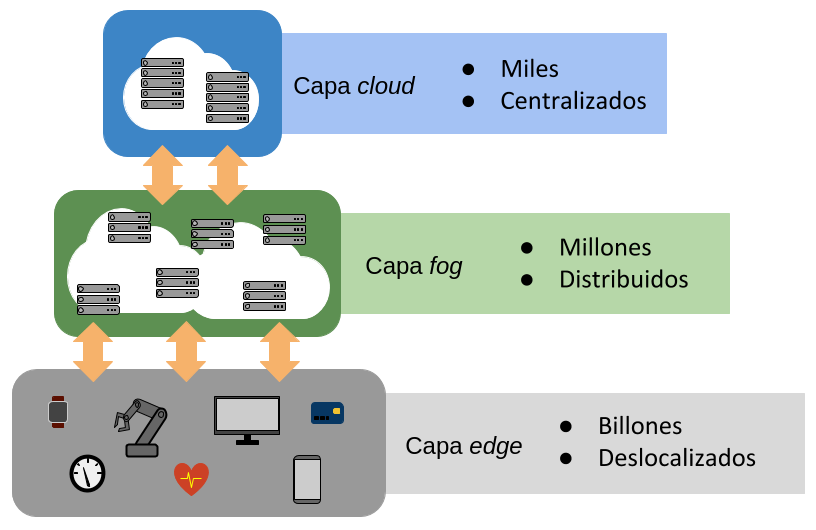
\includegraphics[width=0.7\textwidth]{02-state_of_the_art/cloud-fog-edge.png}
  \caption{Estructura por capas \textit{cloud-fog-edge}}
  \label{fig:02-cloud_fog_edge}
\end{figure}

Dejando atrás la ya explicada nube, vamos a adentrarnos más en el \textit{fog}.
Esta capa se compone de los llamados nodos \textit{fog}, que son los encargados
de llevar a cabo las distintas tareas. Cualquier dispositivo con capacidad de
procesamiento, memoria y conexión de red puede ser un nodo viable. De esta
forma, se pueden usar como nodos routers, switches y otros dispositivos de
redes, así como cámaras de videovigilancia. Se aprovecha la capacidad de
procesamiento de todos estos dispositivos cuando no se están usando al 100\%.
Como ya se ha indicado, estos nodos se encuentran ubicados en la misma red local
(LAN) que los dispositivos del borde de la red que generan los datos. Las
distintas tareas de análisis y control a realizar sobre estos datos se
distribuyen sobre los nodos \textit{fog} de forma dinámica dependiendo de la
carga de trabajo que posean los mismos. A la hora de asignar una tarea a un
nodo, siempre se debe intentar hacer de forma que el nodo elegido esté lo más
cerca posible de la fuente de los datos \cite{gedeon_fog_2018}. Esto es
especialmente importante para tareas de control, donde es posible que no todos
los nodos \textit{fog} de la planta tengan la latencia necesaria para cumplir
con los requisitos temporales. En este sentido, en \cite{pop_enabling_2018} se
propone el uso de TSN (\textit{Time-Sensitive Networking}) para las
comunicaciones en la capa \textit{fog}, con el objetivo de reducir estas
latencias. Este modelo de computación distribuida sobre una bolsa o
\textit{pool} de recursos es muy similar al que encontramos en la nube, con la
diferencia de que en el \textit{fog} estos recursos son mucho más limitados, por
lo que es también esencial optimizar el uso de los mismos. Debido a esta
similitud con el modelo de la nube, las mismas tecnologías de virtualización
usadas en ésta también son útiles en el nuevo paradigma \cite{yi_fog_2015}.
Algunos modelos ya han sido propuestos para la aplicación del \textit{fog} a los
sistemas industriales y el modelado de la Industria 4.0
\cite{verba_modeling_2019} \cite{tseng_lightweight_2018}.

Aunque la capacidad de procesamiento del \textit{fog} es mucho menor que la de
la nube, sigue siendo útil para realizar algunas tareas menos intensivas
evitando tener que desplazar todos los datos a la nube, con la latencia y la
carga en la red que eso supone. Como consecuencia del avance del IoT
(\textit{Internet of Things}) industrial, que es considerada una de las
tecnologías más importantes para la Industria 4.0 \cite{lu_industry_2017}, el
número de dispositivos presentes en las plantas y, por tanto, la cantidad de
datos que se generan va a ser mucho mayor, poniendo aún más presión sobre la
red, que es donde se podría producir el cuello de botella \cite{shi_edge_2016}.
El \textit{edge} trata de solucionar esto al reducir la cantidad de datos que se
deben enviar hacia las capas superiores procesando una parte de ellos de forma
local. Cabe destacar que el \textit{fog} también permite relajar el tráfico de
red \cite{wang_traffic_2019}. Los dispositivos del borde de la red, aún
ofreciendo menos potencia que la combinada del \textit{fog}, también pueden ser
usados para realizar algunas acciones sobre los datos. En concreto, las tareas
de control que requieran de un tiempo de respuesta más rápido pueden realizarse
en esta capa, tomando decisiones directamente sobre los datos que recoge el
dispositivo. Por otra parte, Khan \cite{khan_edge_2019} identifica la falta de
confianza en los sistemas \textit{edge} como uno de los principales problemas a
los que se enfrenta el paradigma, además de la integración de sistemas y la
movilidad. Esta falta de confianza es especialmente grave si pretendemos
desplegar sistemas de control críticos sobre plataformas de este tipo. Como
solución al problema de la confianza, Stanciu \cite{stanciu_blockchain_2017}
propone usar tecnología de \textit{blockchain} para desplegar sistemas de
control distribuidos en el \textit{edge}.

Sectores como el automovilístico, energético o de alimentación están muy
interesados en el desarrollo de la Industria 4.0 debido a los importantes
beneficios que se estima que puede tener para sus procesos. Gracias al 5G y a
las mejoras en las comunicaciones, el IoT se convierte en una idea capaz de dar
a las organizaciones una cantidad de información sobre sus procesos industriales
jamás vista antes. Estos datos son la base de la Industria 4.0
\cite{khan_perspective_2016}, ya que permiten la definición de sistemas
ciber-físicos y gemelos digitales que replican perfectamente los procesos
físicos en el plano digital, lo que abre la puerta a un control inédito sobre
dichos procesos. Además de las comunicaciones, otro reto muy importante para la
consecución de estos objetivos es el modelado de estos sistemas cuidando los
aspectos deseados de seguridad y fiabilidad \cite{farsi_industry_2019}. En este
sentido, creemos que el \textit{fog} es un modelo de computación que puede
facilitar el diseño de estos CPS al proporcionar una plataforma robusta y
unificada sobre la que implementarlos.

\section{Tecnologías de virtualización: hipervisores y contenedores}

De manera simple, la virtualización consiste en abstraer ciertas capas de un
sistema convencional (p. ej., el hardware). Sobre estas abstracciones se pueden
ejecutar procesos o sistemas completos de manera aislada. Este aspecto es el que
hace de la virtualización un concepto tan relevante para la computación en la
nube, ya que posibilita el acceso compartido a los recursos. Por ejemplo, sobre
una misma CPU se podrían ejecutar varios sistemas operativos completamente
funcionales de forma que ninguno de ellos sepa de la existencia de los otros.
Cada uno de estos sistemas cree que tiene una CPU completa para él gracias a la
abstracción del hardware. Aunque las tecnologías de virtualización han
experimentado un empuje enorme en los últimos años debido a la expansión de la
nube, no se trata de una idea novedosa. En 1974, Popek y Goldberg
\cite{popek_formal_1974} definían los requisitos que debía cumplir una
plataforma para poder virtualizar sistemas completos. Hoy en día, hablamos de
virtualización en dos niveles diferentes: a nivel del hardware (máquinas
virtuales) o a nivel del sistema operativo (contenedores).

Lo que se quiere decir con virtualización a nivel del hardware, es que es éste
el que se abstrae. Esto es precisamente lo que sucede con las máquinas
virtuales. El hardware «real» se puede fraccionar para asignarlo a las diversas
máquinas virtuales, que lo usan como si se tratase de una plataforma física
normal y corriente. Así, se puede regular la cantidad de CPU, memoria RAM o,
incluso, acceso a dispositivos de I/O que tiene cada máquina virtual. Todo esto
es posible gracias a los hipervisores, que son la pieza de software encargada de
abstraer el hardware y regular su uso por parte de las máquinas virtuales.
Dependiendo de la relación existente entre el hipervisor y el hardware que
abstraen, nos encontramos con hipervisores de tipo 1 y 2. Un hipervisor de tipo
2 se ejecuta sobre un sistema operativo tradicional, que recibe el nombre de
anfitrión, mientras que los de tipo 1 prescinden del anfitrión, ejecutándose
directamente sobre el hardware que gestionan (\textit{bare metal}). En la figura
\ref{fig:02-hypervisors} se representa gráficamente esta diferencia.

\begin{figure}
  \centering
  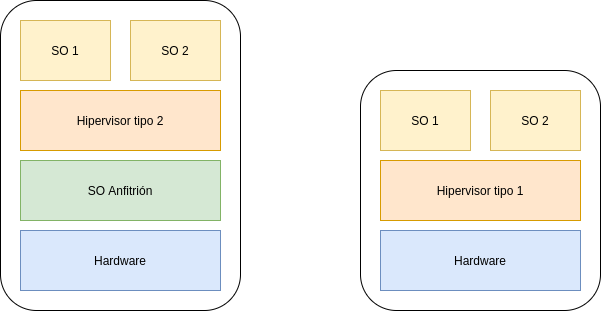
\includegraphics[width=0.8\textwidth]{02-state_of_the_art/hypervisors.png}
  \caption{Capas de la virtualización mediante hipervisores de tipo 1 y 2}
  \label{fig:02-hypervisors}
\end{figure}

Como es obvio, los hipervisores de tipo 1 suponen una solución mucho más liviana
que los de tipo 2 al no tener un anfitrión. Por otra parte, pueden asignar
prácticamente todos los recursos hardware de la plataforma a las máquinas
virtuales de forma dinámica, mientras que los de tipo 2 se ven restringidos a
los límites impuestos por el anfitrión. Los hipervisores de tipo 2 son más
utilizados en el ámbito personal, con herramientas como VirtualBox o VMWare
siendo muy utilizadas para la prueba de software, mientras que los de tipo 1 son
los que predominan a nivel empresarial e industrial, con claros ejemplos como
PikeOS o Xen. Este último supuso un importante avance en la ejecución segura y
aisla de máquinas virtuales sobre hardware de uso común \cite{barham_xen_2003}.
En lo que a sistemas de tiempo real se refiere, RT-Xen \cite{xi_rt-xen_2011} se
presentó como un marco de referencia para la planificación de procesos con
restricciones temporales en sistemas Linux virtualizados usando Xen, obteniendo
prometedores resultados.

Mientras que en la virtualización a nivel del hardware las máquinas virtuales
contienen un sistema operativo completo, en la virtualización a nivel del
software solo se virtualizan procesos. Estos procesos virtualizados, que reciben
comúnmente el nombre de contenedores, acceden a los servicios básicos del
sistema operativo anfitrión. De forma análoga a los hipervisores, los motores de
contenedores son los encargados de gestionar los procesos y su acceso al sistema
operativo que comparten. Realmente, los procesos contenerizados se ejecutan
sobre el sistema anfitrión como lo harían los procesos «nativos». La única
diferencia se encuentra en que los procesos contenerizados están aislados del
resto. Estos procesos solo pueden ver al resto de procesos de su mismo
contenedor, no los del resto de contenedores ni los no contenerizados. Para
conseguir este aislamiento, los motores de contenedores aprovechan varias
características del kernel de Linux, entre las que destacamos:

\begin{itemize}
  \item Espacios de nombres (\textit{namespaces}): los identificadores de
        proceso (PID), las interfaces de red o la parte del sistema de ficheros que
        puede ver un proceso contenerizado depende del espacio de nombres al que se
        asigne cuando se crea. Usando esta herramienta, se puede restringir lo que ven
        los contenedores del sistema anfitrión.
  \item Grupos de control (\textit{control groups}): Los \texttt{cgroups} son
        mecanismos que permiten regular el acceso al hardware por parte de los
        contenedores, así como su acceso compartido.
\end{itemize}

A primera vista, cabría pensar que, dado que contienen un sistema operativo
completo, las máquinas virtuales son mucho más pesadas que los contenedores. No
obstante, en trabajos como \cite{manco_my_2017} \cite{felter_updated_2015} se
desmiente esta percepción. Concretamente, en el último se compara el popular
motor de contenedores Docker con KVM, un famoso hipervisor para Linux, llegando
a la conclusión de que ninguno de los dos penaliza de manera significativa el
rendimiento en cuanto a uso de CPU o memoria, si bien es cierto que las máquinas
virtuales de KVM obtenían peores resultados en las operaciones de I/O. Por otro
lado, la seguridad en los contenedores es un aspecto todavía en desarrollo
\cite{randal_ideal_2020}, sobre todo en la seguridad del kernel compartido.

Existen múltiples motores de contenedores usados ampliamente en la actualidad,
como es el caso de Docker, Rocket (rkt) o LXC (\textit{LinuX Containers}).
Kozhirbayev y Sinnot \cite{kozhirbayev_performance_2017} realizaron en 2017 una
comparativa del rendimiento entre Docker y LXC\footnote{Concretamente, se hace
  uso de Flockport.}. Los resultados obtenidos coinciden con los vistos en
\cite{felter_updated_2015} en tanto que los procesos contenerizados no tienen
una penalización en el consumo de CPU o RAM frente a los nativos, aunque sí que
se observa esta penalización en las operaciones de I/O. Como el rendimiento es
similar para todos los motores de contendores, se ha decidido poner el foco
sobre Docker para este trabajo debido a que es el más popular, con el
consecuente impacto que esto tiene en la calidad del soporte y de la
documentación disponible.

\begin{figure}
  \centering
  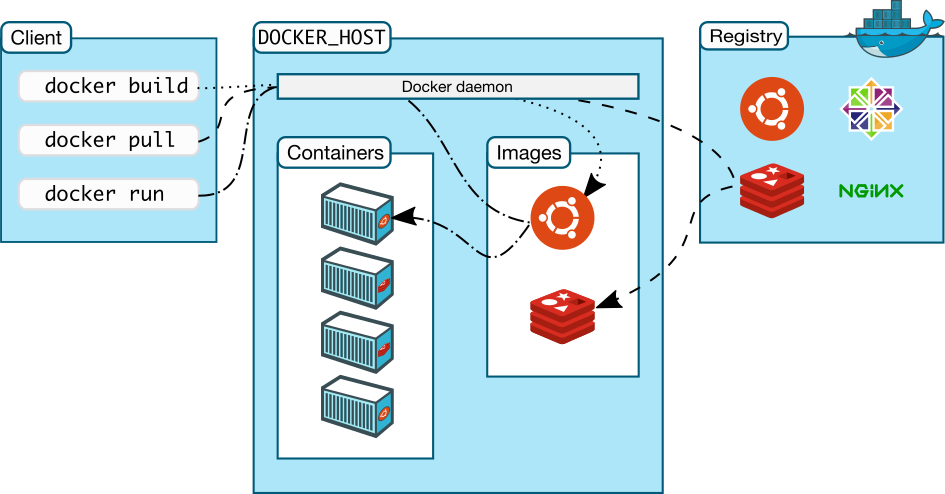
\includegraphics[width=\textwidth]{02-state_of_the_art/docker.png}
  \caption{Esquema de funcionamiento de Docker}
  \label{fig:02-docker}
\end{figure}

En Docker, al igual que en muchos otros motores de contenedores, los
contenedores se lanzan a partir de imágenes, definidas mediante un
\texttt{Dockerfile}. Una imagen es reutilizable y universal, pudiendo lanzar
réplicas de un mismo contenedor en cualquier plataforma soportada por la imagen.
Para trabajar con imágenes y contenedores, el sistema Docker se compone de dos
partes principales: el demonio\footnote{Un demonio o \textit{daemon} es un tipo
  de proceso que se ejecuta en segundo plano para ofrecer un servicio.} y el
cliente. El demonio es el encargado de realizar todas las soperacones
relacionadas con imágenes o contenedores, incluyendo su construcción,
lanzamiento y gestión posterior. Para realizar estas acciones, expone una API
con la que pueden interactuar los distintos clientes, siendo el oficial que
proporciona Docker una aplicación de línea de comandos. A estos dos componentes
se podría añadir un tercero, el registro de imágenes. Como su propio nombre
indica, se trata de una especie de base de datos de imágenes listas para su uso.
De esta forma, se pueden almacenar y compartir imágenes entre varios
dispositivos a través de la red. No obstante, se puede hacer uso de Docker de
manera local sin necesidad de usar un registro externo. Un esquema del
funcionamiento de Docker que se acaba de explicar se puede ver en la figura
\ref{fig:02-docker}.

Centrando nuestra atención de nuevo en los sistemas de control industrial, se
plantea la posibilidad de implementarlos usando contenedores
\cite{hofer_industrial_2019}, aunque los principales inconvenientes
identificados son los relacionados con la seguridad. En
\cite{cinque_rt-cases_2019}, los autores proponen un modelo de planificación de
procesos contenerizados para conjuntos de tareas con distintos niveles de
criticalidad, defendiendo el uso de contenedores por su capacidad de
aislamiento. Sin embargo, en la encuesta sobre contenerización para tiempo real
realizada por Struhár et al. en 2020 \cite{struhar_real-time_2020}, se llega a
la conclusión de que son necesarias mejores herramientas para la gestión de
contenedores de tiempo real. Por ello, en este trabajo se plantea el desarrollo
de una herramienta para este fin como prueba de concepto. Los autores del
estudio destacan también la falta de un mecanismo determinista de comunicación
entre procesos contenerizados y de herramientas de validación y prueba, además
de los problemas de seguridad ya mencionados.

\section{Aspectos de computación en tiempo real: RTOS, algoritmos de
  planificación y herramientas}
\label{sec:real-time}

En esta sección, se va a explicar con mayor detalle el funcionamiento de los
sistemas de tiempo real ya mencionados en las secciones anteriores. En estos
sistemas, el tiempo es un factor crucial a la hora de determinar la validez de
las salidas. De esta forma, las tareas ejecutadas se ven limitadas por
restricciones temporales. Dependiendo de la severidad de las consecuencias del
incumplimiento de las restricciones, solemos hablar de tareas y restricciones
duras o blandas. Las restricciones duras son aquellas que, si se incumplen,
tienen consecuencias son muy graves, como pueden ser daños a la vida de las
personas en el caso de sistemas que sean críticos. En cuanto a las restricciones
blandas, solo se experimenta una pérdida de calidad en el servicio cuando se
incumplen, aunque se suele limitar el número de incumplimientos permitido. En la
figura \ref{fig:02-deadlines} se muestra la diferencia entre los dos tipos de
restricciones según su función de utilidad \cite{wang_introduction_2013}, que es
la que define el valor de la salida del sistema en función del tiempo. Como se
puede apreciar, el resultado de una tarea dura solo es útil si se da entre el
inicio de la tarea y su límite temporal fijado, provocando daños de cualquier
otra manera. En las tareas blandas, el resultador puede tener valor incluso si
se obtiene después del límite, aunque se va reduciendo con el tiempo.

Debido a la gran responsabilidad que recae sobre el cumplimiento de estos
requisitos, los sistemas empotrados sobre los que se ejecutan estas tareas
tienen características diferentes a las de los sistemas de uso general. A nivel
del hardware, por ejemplo, las CPU tienen un diseño más simple que haga más
fácil verificar el determinismo en sus operaciones. En
\cite{rotenberg_chapter_2005}, Rotenberg y Anantaraman describen el
funcionamiento de las CPU de alto rendimiento y las comparan con las empotradas.
La ejecución predictiva, por ejemplo, es severamente limitada en los sistemas
empotrados. Por otro lado, las operaciones de acceso a caché y RAM suponen están
optimizadas para necesitar un menor número de ciclos. Normalmente, el conjunto
de instrucciones (ISA) de estas CPU es reducido, conocido como RISC, reduciendo
la complejidad y facilitando la programación a bajo nivel. ARM es una de las
arquitecturas de microprocesador basadas en RISC más usadas para el diseño de
sistemas empotrados. Otro aspecto diferencial es el número de núcleos o
\textit{cores} presentes en los procesadores. Poseer varios núcleos hace posible
la ejecución en paralelo de instrucciones, mejorando el rendimiento en los
sistemas. No obstante, este paralelismo dificulta asegurar el determinismo,
aunque algunos algoritmos de planificación de procesos han sido propuestos
\cite{anderson_edf-based_2005} y la investigación es activa en este área. Para
asegurar además que las tareas se puedan ejecutar correctamente, los sistemas de
tiempo real suelen dejar capacidad de CPU extra libre.

\begin{figure}
  \centering
  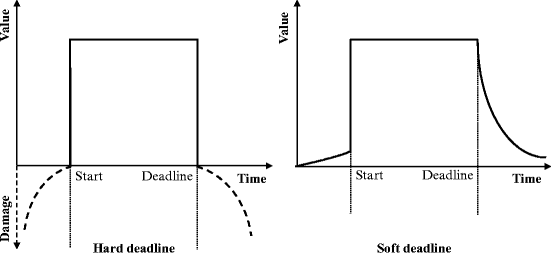
\includegraphics[width=0.8\textwidth]{02-state_of_the_art/deadlines.png}
  \caption{Funciones de utilidad para restricciones temporales duras y blandas}
  \label{fig:02-deadlines}
\end{figure}

Además del hardware, el software usado para implementar estos sistemas también
es especial. Los lenguajes y herramientas deben proporcionar al programador
ciertas comodidades para la implementación de procesos en tiempo real
\cite{burns_real-time_2009}:

\begin{itemize}
  \item Especificar momentos en los que las acciones se deben realizar.
  \item Especificar los momentos antes de los cuales las acciones deben terminar.
  \item Permitir la ejecución repetitiva (periódica y aperiódica) de trabajo.
  \item Limitar la varianza en las operaciones de entrada y salida.
  \item Responder a situaciones donde no todas las restricciones temporales se
        pueden cumplir.
  \item Responder a situaciones en las que los requisitos de tiempo cambian de
        manera dinámica.
\end{itemize}

Una parte muy importante de los sistemas empotrados es su sistema operativo, el
cual gestiona los recursos físicos de la plataforma y controla el uso de los
mismos por parte de los procesos implementados por los desarrolladores. Al igual
que ocurre con el hardware, estos sistemas operativos también tienen
características diferentes a los de propósito general para poder dar cobijo a
tareas con restricciones temporales, recibiendo el nombre de RTOS (\textit{Real
  Time Operating System}). La principal diferencia, podríamos decir que se
encuentra en los algoritmos de planificación de tareas usados, aunque cabe
destacar que también hay otras áreas importantes como el acceso a memoria o la
gestión de las interrupciones. El algoritmo de planificación es, a grandes
rasgos, la política que decide en qué orden se ejecutan las tareas del sistema.
En los sistemas normales, normalmente se asigna a cada proceso una fracción
igualitaria de tiempo de CPU, ejecutándose hasta que consume su fracción de
tiempo o se bloquea (p. ej., por una operación de lectura o escritura). En los
sistemas de tiempo real, este método no es factible, ya que los procesos tienen
distintas prioridades y no pueden quedar a la espera de que otro proceso de
menor prioridad libere la CPU. Por ello, la planificación de procesos de tiempo
real es apropiativa (\textit{preemptive scheduling}), de forma que el sistema
operativo puede quitar la CPU a un proceso que está en ejecución para
asignársela a otro más prioritario. Como se destaca en
\cite{burns_scheduling_1991}, la planificación de procesos óptima para un
sistema de tiempo real «duro» depende enormemente del problema en cuestión. ¿Se
trata de un sistema uniprocesador o multiprocesador? ¿Todas las situaciones son
conocidas de antemano? ¿Las tareas son periódicas o aperiódicas? Dependiendo de
la situación, podemos encontrarnos con que un algoritmo de planificación es más
eficaz que otro.

Antes de entrar a explicar algunos de los algoritmos de planificación de tareas
más importantes, debemos entender mejor como son estas tareas. Las tareas en un
sistema de tiempo real pueden ser provocadas por tiempo o por eventos. Las
tareas provocadas por tiempo son tareas periódicas, con un tiempo definido para
sus ciclos. Las caracterizamos con los siguientes atributos:

\begin{itemize}
  \item Tiempo de ejecución $WCET$ (\textit{Worst Case Execution Time}): Se trata
        del tiempo que se necesita para completar la tarea en el peor caso.
  \item Límite de tiempo $D$ (\textit{Deadline}): Momento temporal posterior a
        la activación de la tarea y antes del cuál se debe haber completado.
  \item Período $T$ (\textit{Period}): Es el tiempo que transcurre entre
        activaciones.
\end{itemize}

Estas tareas son ejecutadas por un reloj interno del sistema, el cuál debe ser
lo suficientemente preciso como para asegurar que los ciclos se cumplen. Por
otra parte, las tareas también pueden ser aperiódicas si son activadas por un
evento externo (p. ej., un cambio en el entorno, como sucede en algunos sistemas
de control) mediante mecanismos como las interrupciones. Las tareas aperiódicas
siguen teniendo $WCET$ y $D$, pero no tienen período $T$. En algunos casos,
existe un tiempo mínimo entre activaciones $T$, considerándose la tarea como
esporádica. En ocasiones, los sistemas empotrados limitan su arquitectura para
que solo haya tareas activadas por tiempo, evitando las interacciones y
comprobando de forma periódica si se ha producido un evento. De todos estos
atributos, el tiempo de ejecución en el peor caso es el más difícil de
determinar. Se trata de un límite superior que puede ser estimado usando métodos
estáticos, probabilísticos o, incluso, basados en mediciones. No obstante, la
fiabilidad de muchos de estos métodos se apoya en supuestos sobre el sistema y
su funcionamiento \cite{abella_wcet_2015}.

Para evaluar la efectividad de un algoritmo de planificación, solemos basarnos
en su capacidad para cumplir con todas las restricciones temporales de un
conjunto de tareas dado. Cuando se consiguen respetar todas estas restricciones,
se dice que la planificación (o el conjunto de tareas) es viable, mientras que
si el sistema se salta alguna, se suele decir que está sobrecargado. Un concepto
muy importante en el que se apoyan los algoritmos de planificación para
determinar la viabilidad de un conjunto de tareas es la utilización total de CPU
para dicho conjunto, definida como

\begin{equation}
  U = \sum_{i=1}^{n} \frac{C_{i}}{min(D_{i}, T_{i})}
\end{equation}

por Liu y Layland \cite{liu_scheduling_1973}, donde $C_{i}$, $D_{i}$ y $T_{i}$
son el tiempo de ejecución, límite temporal y período para la tarea $i$ del
conjunto, respectivamente.

Anteriormente, se ha indicado que la planificación de procesos de tiempo real es
apropiativa, de forma que el sistema operativo puede retirarle a un proceso los
recursos que tenía asignado para dárselos a otro de mayor prioridad. La
asignación de estas prioridades a las distintas tareas es la base de los
algoritmos de planificación. Estos algoritmos pueden ser de dos tipos: estáticos
o dinámicos. Los algoritmos estáticos realizan la planificación y asignan las
prioridades a las tareas antes incluso de tener que poner en marcha el sistema,
de forma \textit{offline}, ejecutándose luego las tareas en el orden determinado
por las prioridades establecidas. También conocida como planificación de
prioridades fijas FPS (\textit{Fixed-Priority Scheduling})
\cite{tilborg_fixed_1991}, para aplicar estos algoritmos es necesario conocer
todas las características del problema de planificación (número de tareas y sus
atributos) de antemano, lo cuál es imposible en algunas situaciones en las que
se desconoce la carga de trabajo futura del sistema. Uno de los algoritmos
estáticos más conocidos es RMS (\textit{Rate Monotonic Scheduling})
\cite{liu_scheduling_1973}\cite{kao_rate-monotonic_2008}, cuya idea principal es
que las tareas con los períodos más pequeños tienen mayor prioridad. En la
propuesta original de RMS realizada por Liu y Layland, asumen un conjunto de
tareas periódicas con $D=T$ y determinan el límite superior para la utilización
como

\begin{equation}
  U \leq n(2^{\frac{1}{n}} - 1)
\end{equation}

Esto implica que, para conjuntos de tareas muy grandes ($n \rightarrow \infty$),
la utilización de CPU tiene que ser inferior al 70\%, que es una cifra
relativamente baja. No obstante, si se cumplen todas estas condiciones, RMS
garantiza encontrar una planificación viable si es que existe, o lo que es lo
mismo, es un algoritmo óptimo. Otro problema de RMS es que requiere que el
período sea igual al límite de tiempo para cada tarea. Para solucionar este
problema, se propone DMT (\textit{Deadline Monotonic Scheduling})
\cite{audsley_hard_1991}, en el que los procesos se caracterizan con $C_{i} \leq
  D_{i} \leq T_{i}$.

Como ya se ha comentado, el principal problema de la planificación estática es
que se trata de algoritmos clarividentes, es decir, necesitan conocer toda la
información sobre el conjunto de tareas para poder determinar su viabilidad. Los
algoritmos dinámicos, por otra parte, permiten determinar esta viabilidad
en tiempo de ejecución, cambiando las prioridades de las tareas sobre la marcha
u \textit{online}. Uno de los algoritmos dinámicos más conocidos es EDF
(\textit{Earliest Deadline First}) \cite{liu_scheduling_1973}, donde las tareas
con menor tiempo restante antes de su límite temporal son las que reciben una
mayor prioridad. En este caso, el algoritmo es óptimo para conjuntos de tareas
donde se cumpla la condición \cite{zhang_schedulability_2009}

\begin{equation}
  U \leq 1
\end{equation}

No obstante, esta situación se da solo en los sistemas uniprocesador. En los
multiprocesador, determinar que la utilización es inferior al número de CPU no
es una condición suficiente para garantizar que el conjunto de tareas tenga una
planificación viable. En 2005, Anderson adapta EDF para sistemas multiprocesador
\cite{anderson_edf-based_2005}, consiguiendo una condición suficiente para
tareas de tiempo real blandas. Un enfoque diferente al de EDF lo proporciona MUF
(\textit{Maximum Urgency First}) \cite{stewart_real-time_1991}. En este
algoritmo, se trabaja en torno a la urgencia de cada tarea, que es determinada
según la combinación de varias prioridades. En concreto, cada tarea posee 2
prioridades fijas definidas antes de la ejecución y una dinámica, que se calcula
sobre la marcha, existiendo una relación de precedencia entre estas prioridades.

En el caso de ser necesario trabajar con tareas aperiódicas o esporádicas, se
puede aplicar alguno de los algoritmos propuestos en
\cite{sprunt_scheduling_1989}, entre los que destacamos DSA (\textit{Deferrable
  Server Algorithm}) y SSA (\textit{Sporadic Server Algorithm}).

Para terminar con el repaso de la computación de tiempo real, vamos a hacer un
breve repaso de algunos de los RTOS más utilizados. En
\cite{hambarde_survey_2014}, Hambarde realiza una comparación entre Windows CE,
VxWorks, QNX Neutrino y RTAI. El último, que es esencialmente una extensión del
kernel de Linux o co-kernel que da soporte a este tipo de cargas de trabajo,
obtiene los mejores resultados en latencia, \textit{jitter} y tiempo de
respuesta de entre los cuatro, si bien es cierto que su latencia ante
interrupciones es mayor que la de VxWorks. Además de RTAI, otros co-kernels para
Linux serían RTLinux y Xenomai. Todos estos co-kernels funcionan de manera
similar: implementan un despachador de interrupciones que captura las
interrupciones provenientes del hardware para redirigirlas a los procesos (tanto
normales como de tiempo real), mientras que también poseen un planificador de
procesos para asegurar que se cumplen las prioridades.

Además de los co-kernels, otra solución alternativa para Linux la encontramos en
el parche \texttt{PREEMPT\_RT}. El desarrollo de este parche es llevado a cabo
por programadores del kernel dentro de la fundación Linux y en paralelo con el
del propio kernel, lo que le da un cierto aire de «oficialidad». En esencia, los
cambios que aplica este parche sobre el kernel habilitan la planificación
apropiativa y aumentan el determinismo de ciertas operaciones. Este
acercamiento, al trabajar sobre un único kernel en vez de los dos que se
obtienen con las soluciones basadas en co-kernels, resulta en una mayor
facilidad a la hora de implementar procesos de tiempo real, ya que se realiza de
manera idéntica a los normales. Los co-kernels exponen interfaces especiales que
se salen de la interfaz estándar de Linux y con las que sus procesos deben
trabajar, algo que no ocurre con el parche \texttt{PREEMPT\_RT} y que hace que
sea muy fácil adaptar un proceso existente para que tenga un comportamiento más
determinista. Este parche habilita varios modos de planificación de procesos
nuevos para el planificador del kernel, entre los que destacaremos
\texttt{SCHED\_DEADLINE} \cite{noauthor_deadline_nodate}. Esta política de
planificación aplica el algoritmo EDF junto con CBS (\textit{Constant Bandwith
  Server}). El algoritmo CBS se encarga de asignar un ancho de banda a cada tarea,
de forma que una tarea concreta no pueda ejecutarse durante un tiempo superior a
su tiempo de ejecución dentro de cada período. De esta forma, se consigue el
aislamiento temporal de las tareas, evitando que el comportamiento de una de
ellas afecte a las demás. En cuanto a su rendimiento, el estudio llevado a cabo
en \cite{reghenzani_real-time_2019} determina que no es una solución apta para
sistemas de tiempo real duro, pero puede ser perfectamente usado cuando las
restricciones son más livianas. En cualquier caso, el rendimiento va a depender
enormemente del hardware utilizado y de la implementación de los drivers para
dicho hardware.

Para este trabajo, se ha decidido usar como plataforma objetivo
el sistema GNU/Linux parcheado con \texttt{PREEMPT\_RT} debido a que se adhiere
a la interfaz estándar del kernel y las tecnologías de virtualización mediante
contenedores presentes en la plataforma son muy maduras. El hecho de que no sea
un RTOS aceptable para sistemas con restricciones temporales duras nos es
indiferente para el alcance de este proyecto, dado que solo se busca implementar
una herramienta que sirva como prueba de concepto de las ideas planteadas.
\chapter{Análisis del rendimiento de procesos contenerizados}
\label{ch:03-performance_analysis}

A lo largo del capítulo anterior se han tomado varias decisiones respecto a las
tecnologías que se van a utilizar en el proyecto. El uso de Linux como
plataforma para la ejecución de tareas de tiempo real parte del objetivo
propuesto para este trabajo de analizar las soluciones de tiempo real basadas en
este kernel. Dentro de estas soluciones, aunque las de mayor rendimiento son las
basadas en co-kernels (p. ej., Xenomai y RTAI), hemos optado por usar el parche
\texttt{PREEMPT\_RT}, que aporta las capacidades de tiempo real al propio kernel
de Linux, apoyando nuestra elección en su adherencia a la interfaz estándar del
kernel y la posibilidad de usar las tecnologías de virtualización más conocidas
del mercado. En la sección \ref{sec:02-virtualization} se comprobaba que el
rendimiento de los distintos motores de contenedores es similar, de forma que
decidimos usar Docker para la virtualización de los procesos de tiempo real
debido a ser el motor más maduro y popular.

Una vez definida esta configuración, hemos decidido evaluar su rendimiento
realizando una serie de pruebas. Dado que el rendimiento de Linux con
\texttt{PREEMPT\_RT} es un aspecto que ya ha sido estudiado enormemente en la
bibliografía, nuestro objetivo es más bien analizar el uso de Docker sobre esta
plataforma. Nuestras pruebas se han realizado sobre el dispositivo Raspberry Pi
detallado en la sección \ref{sec:01-tools}. Debido a sus características, la
Raspberry Pi es un dispositivo muy similar a los que nos podríamos encontrar en
una hipotética capa \textit{edge}, de forma que nos sirve para obtener unos
resultados orientativos del rendimiento que se podría obtener en este entorno.

Existen múltiples proyectos comunitarios enfocados a proporcionar utilidades
para la prueba de las características de tiempo real del kernel de Linux, como
es el caso del \textit{Linux Test Project}. Se trata de un conjunto de casos de
prueba para validar la fiabilidad, robustez y estabilidad de Linux, con algunos
orientados a los aspectos de computación en tiempo real. Otro ejemplo lo tenemos
en la suite de pruebas \texttt{rt-tests}, que recoge una serie de programas o
\textit{benchmarks} especialmente centrados en las políticas de planificación de
tiempo real. Hemos decidido usar esta suite en lugar de LTP u otras alternativas
debido a la presencia del programa de prueba \texttt{cyclicdeadline}, que es un
derivado del conocido \texttt{cyclictest}. El objetivo de estos dos programas es
evaluar la latencia en la activación de procesos de tiempo real, es decir, la
diferencia de tiempo entre el momento en el que se debería activar una tarea y
en el que se activa realmente. En \texttt{cyclictest}, esto se hace definiendo
un número determinado de hilos a los que se asignan prioridades diferentes para
ser planificados con la política \texttt{SCHED\_FIFO}. Estos hilos se activan de
forma periódica y se registran las latencias. La principal diferencia que
incorpora \texttt{cyclicdeadline} es el uso de tareas verdaderamente periódicas
planificadas con \texttt{SCHED\_DEADLINE}. Se mide entonces la latencia en la
activación de las tareas para cada período. Como se ha indicado en la sección
\ref{sec:02-real_time}, esta última es la política de planificación elegida para
el sistema que se desea desarrollar, razón por la cuál hemos decidido usar
\texttt{cyclicdeadline} en busca de unos resultados que sean más representativos
del uso real que tendrá el sistema.

Concretamente, se han hecho varias ejecuciones de esta prueba aumentando cada
vez el número de hilos de tiempo real que se debían ejecutar y observar para
poner una carga mayor sobre el procesador y aumentar la complejidad de la
planificación. Para todos los hilos, el límite de tiempo o \textit{deadline} ha
sido de 1000$\mu s$. Estas pruebas se han realizado dos veces: primero,
ejecutando \texttt{cyclicdeadline} de forma «nativa» y, luego, dentro de un
contenedor. La definición de la imagen Docker que contiene la prueba, así como
los pasos seguidos para su ejecución, son explicados detalladamente en el
apéndice \ref{app:C-container_tests}. Los resultados obtenidos son los mostrados
en la tabla \ref{tab:03-cyclicdeadline_latency}. Cabe destacar que
\texttt{cyclicdeadline} solo nos devuelve al final de su ejecución, para cada
uno de los hilos, los valores mínimo, máximo y medio de la latencia. Por ello,
los resultados de la tabla para ejecuciones con más de un hilo muestran
realmente el mínimo de los mínimos de los hilos, el máximo de los máximos y la
media de las medias.

\begin{table}
    \centering
    \begin{tabular}{ | c | c | c | c | c | }
        \hline
                      &                & \textbf{Latencia}         & \textbf{Latencia}         & \textbf{Latencia}        \\
        \textbf{Tipo} & \textbf{Hilos} & \textbf{mínima ($\mu s$)} & \textbf{máxima ($\mu s$)} & \textbf{media ($\mu s$)} \\
        \hline
        Contenedor    & 1              & 1                         & 113                       & 22.0                     \\
        \hline
        Contenedor    & 2              & 1                         & 257                       & 85.0                     \\
        \hline
        Contenedor    & 3              & 1                         & 362                       & 127.33                   \\
        \hline
        Contenedor    & 4              & 1                         & 426                       & 112.0                    \\
        \hline
        Contenedor    & 5              & 1                         & 527                       & 210.20                   \\
        \hline
        Contenedor    & 6              & 1                         & 700                       & 263.0                    \\
        \hline
        Nativo        & 1              & 1                         & 88                        & 17.0                     \\
        \hline
        Nativo        & 2              & 1                         & 267                       & 123.0                    \\
        \hline
        Nativo        & 3              & 1                         & 332                       & 149.0                    \\
        \hline
        Nativo        & 4              & 1                         & 307                       & 122.0                    \\
        \hline
        Nativo        & 5              & 3                         & 448                       & 196.0                    \\
        \hline
        Nativo        & 6              & 1                         & 613                       & 205.67                   \\
        \hline
    \end{tabular}
    \caption{Resultados obtenidos de la ejecución de \texttt{cyclicdeadline}.}
    \label{tab:03-cyclicdeadline_latency}
\end{table}

Lo que queríamos observar con estas pruebas es el impacto que tiene sobre la
latencia el uso de Docker. En la gráfica de la figura
\ref{fig:03-cyclicdeadline_latency}, se muestran los datos de la anterior tabla
de forma que este impacto se hace evidente. Aunque la latencia media se mantiene
relativamente similar, el límite superior es mayor en las ejecuciones
contenerizadas. No obstante, el impacto no es especialmente notable, de forma
que se puede seguir considerando como una herramienta factible para el
despliegue de procesos de tiempo real, si bien no será recomendable para los que
tengan unas restricciones temporales más pequeñas donde esta latencia sea
demasiado alta.

\begin{figure}
    \centering
    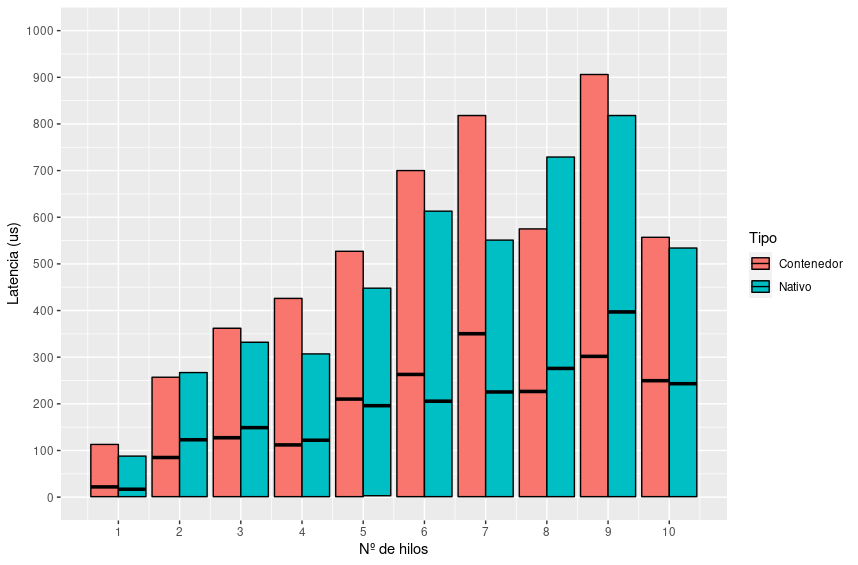
\includegraphics[width=\textwidth]{03-container_analysis/cyclicdeadline-latency.png}
    \caption{Gráfica de intervalos con los rangos de latencia mínima a máxima
        obtenidos de la ejecución de \texttt{cyclicdeadline}. Para cada rango, se
        muestra también su media.}
    \label{fig:03-cyclicdeadline_latency}
\end{figure}

Hay que tener en cuenta que la ejecución de \texttt{cyclicdeadline} dentro de un
contenedor se realiza de forma que este programa lanza los hilos de tiempo real
dentro de su mismo contenedor, el cuál ya se encuentra en ejecución. Por ello,
se decidió realizar una segunda prueba con el objetivo de analizar la latencia
en el lanzamiento de los propios contenedores, dato que es especialmente
importante en el contexto que se plantea para la herramienta de orquestación de
tareas de tiempo real, dado que estas tareas se deben lanzar en los nodos desde
cero. Para que la ejecución del proceso de prueba no influya en los resultados,
se ejecuta todo este proceso desde un ordenador externo «maestro». El
funcionamiento es el siguiente:

\begin{enumerate}
    \item El maestro lanza un contenedor en la Raspberry Pi mediante SSH.
    \item Cuando el contenedor se lanza, envía un mensaje UDP de vuelta al
          maestro informando de que ha terminado su ejecución.
    \item El maestro obtiene los tiempos de creación e inicio del contenedor
          ejecutando el comando \texttt{docker inspect} mediante SSH.
    \item La latencia se obtiene como la diferencia entre ambos tiempos.
    \item El maestro elimina el contenedor de la Raspberry Pi mediante SSH para
          poder lanzarlo de nuevo en la siguiente iteración.
\end{enumerate}

Para comprobar también si el lenguaje usado en la implementación del proceso
contenerizado tiene algún impacto sobre esta latencia, se han usado tres
versiones diferentes del contenedor que se lanza sobre la Raspberry Pi, usando
C, Go y Rust. Los tres son lenguajes compilados con similitudes en cuanto a su
alcance (programación de sistemas) y características. En total, se han realizado
1000 iteraciones de esta prueba para cada uno de los lenguajes. Los resultados
obtenidos se muestran en la tabla \ref{tab:03-container_latency}. En la figura
\ref{fig:03-container_latency} se puede observar una representación gráfica de
todas las latencias observadas para cada iteración.

\begin{table}[H]
    \centering
    \begin{tabular}{ |c|c|c|c|c| }
        \hline
                          & \textbf{Tiempo}        & \textbf{Tiempo}        & \textbf{Tiempo}       & \textbf{Desviación} \\
        \textbf{Lenguaje} & \textbf{mínimo ($ms$)} & \textbf{máximo ($ms$)} & \textbf{medio ($ms$)} & \textbf{típica}     \\
        \hline
        C                 & 1472                   & 2548                   & 1693                  & 165                 \\
        \hline
        Go                & 1445                   & 2718                   & 1693                  & 163                 \\
        \hline
        Rust              & 1478                   & 2378                   & 1701                  & 156                 \\
        \hline
    \end{tabular}
    \caption{Valores observados para la latencia en el lanzamiento de
        contenedores implementados en distintos lenguajes.}
    \label{tab:03-container_latency}
\end{table}

A primera vista, apreciamos que el lenguaje usado para la implementación de los
procesos contenerizados no tiene ningún impacto sobre la latencia en su
lanzamiento. Por otro lado, se trata de valores muy altos, demasiado como para
que podamos considerar el lanzamiento de un contenedor como parte de una tarea
de control estricta. También destaca la gran variación de estas latencias. Todo esto
nos hace pensar que la implementación que tiene Docker de sus tareas de gestión
del ciclo de vida de los contenedores no están preparadas para ser
deterministas, aunque, obviamente, dudamos de que este aspecto fuera considerado
en su diseño.

\begin{figure}
    \centering
    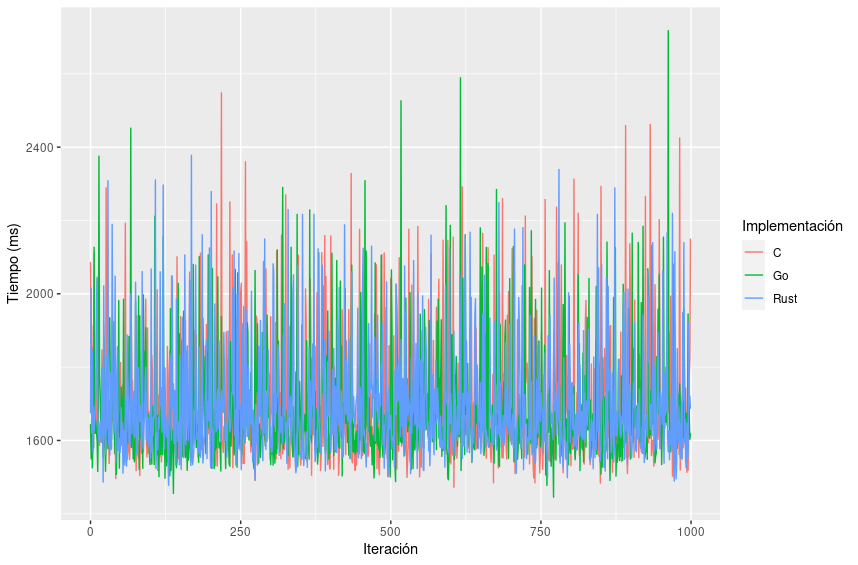
\includegraphics[width=\textwidth]{03-container_analysis/container-latency.png}
    \caption{Gráfico de líneas con las latencias observadas en el lanzamiento de
        contenedores implementados con distintos lenguajes.}
    \label{fig:03-container_latency}
\end{figure}

Sería muy interesante ejecutar estas mismas pruebas usando algún otro motor de
contenedores (p. ej., Podman, Kata, rkt) y así comprobar si, aunque en su
análisis general el rendimiento es similar, en la ejecución de procesos de
tiempo real se observa alguna diferencia. Es más, también se podría probar una
configuración basada en hipervisores para comparar su rendimiento con el de los
contenedores, aunque ya se vió en la sección \ref{sec:02-virtualization} que
éste debería ser parecido \cite{manco_my_2017} \cite{felter_updated_2015}.
\chapter{Diseño e implementación de un orquestador para tareas de tiempo real}

En los capítulos anteriores, se ha presentado el concepto de la Industria 4.0 y
los problemas que plantea, indicando que el paradigma del \textit{fog computing}
y las tecnologías de virtualización pueden ser una solución factible para
conseguir su implantación. Para apoyar este planteamiento, se ha decidido
implementar una herramienta de orquestación de tareas de tiempo real sobre
entornos distribuidos que sirva como prueba de concepto. En este capítulo, se
detalla el proceso seguido para su desarrollo, justificando las decisiones
de diseño tomadas y mostrando los de detalles más relevantes de la
implementación. Para terminar, se muestra una caracterización inicial del
rendimiento de la herramienta desarrollada.

\section{Objetivos y requisitos}

Como ya se ha explicado, la llegada de la Industria 4.0 supone un aumento muy
grande en la cantidad de datos generados en las plantas debido al IoT
industrial, datos que son necesarios para poder obtener gemelos digitales con un
nivel de detalle suficiente. Los nuevos sistemas ciber-físicos necesitan, por
tanto, procesar todos estos datos en tiempo real para poder tomar decisiones de
control en base a los mismos y garantizar una operación eficiente. Para ello, es
necesario poseer una capacidad de procesamiento elevada, mayor de la que
cualquier dispositivo individual pueda aportar. Aunque la computación en la nube
pueda parecer una solución natural a este problema, la enorme carga que pondría
sobre la red la constante transmisión de cantidades de datos tan grandes, así
como la latencia resultante de estas comunicaciones, hacen que no podamos
considerar esta plataforma como apropiada para dar cobijo a tareas con
restricciones temporales. En la sección \ref{sec:02-cloud_fog_edge}, se introduce
el paradigma \textit{fog} como una extensión de la nube más cercana a las
fuentes de datos. Según este modelo, los datos generados por los dispositivos
del borde de la red son procesados en nodos ubicados en la misma red local.
Aunque la potencia combinada de los dispositivos que conformen esta capa
\textit{fog} será menor que la que encontramos en la nube, puede ser suficiente
para las tareas de análisis de datos y toma de decisiones que se deben realizar
en las plantas, reduciendo así la presión sobre la red y garantizando unos
tiempos de respuesta muy inferiores.

Debido a esto, el modelo \textit{fog} se plantea como una posible plataforma
para la implementación de los nuevos sistemas ciber-físicos. Las tareas de
control industrial deben, entonces, distribuirse por los nodos de la capa
\textit{fog} de forma dinámica para dar respuesta a la carga de trabajo en todo
momento. Para que esta distribución de procesos sobre los nodos se produzca de
manera eficiente, es necesario hacer uso de las tecnologías de virtualización,
las cuales ya sirven para solucionar una problemática similar en la nube. Al
virtualizar los procesos, se abstraen las capas inferiores como son el hardware
o el sistema operativo, facilitando el despliegue de los mismos sobre
dispositivos con características dispares y unificando su desarrollo, dado que
no es necesario implementarlos para cada plataforma distinta). Así, se facilita
la escalabilidad de los procesos para dar respuesta a los cambios en la demanda.
En la sección \ref{sec:02-virtualization}, planteamos el uso de contenedores en vez
de máquinas virtuales para esto, apoyándonos en su carácter más liviano y su
mejor rendimiento para operaciones de entrada y salida.

Por tanto, en el modelo planteado es necesario desplegar las tareas de control
en forma de contenedores. Para explorar más este concepto, hemos decidido
implementar una herramienta que permita realizar esto sobre múltiples nodos. Los
objetivos de esta herramienta son:

\begin{table}[H]
    \centering
    \begin{tabular}{ |>{\columncolor[gray]{0.8}}l|p{0.7\textwidth}| }
        \hline
        Nombre      & Gestión de nodos                                       \\
        \hline
        Importancia & Alta                                                   \\
        \hline
        Descripción & Llevar un control de los dispositivos que conforman la
        capa \textit{fog} es una parte esencial de la implantación de este
        modelo.                                                              \\
        \hline
    \end{tabular}
    \caption{Objetivo 01 - Gestión de nodos.}
    \label{tab:04-obj01}
\end{table}

\begin{table}[H]
    \centering
    \begin{tabular}{ |>{\columncolor[gray]{0.8}}l|p{0.7\textwidth}| }
        \hline
        Nombre      & Gestión de tareas                                          \\
        \hline
        Importancia & Alta                                                       \\
        \hline
        Descripción & Las distintas tareas que se deben ejecutar sobre los nodos
        de la capa \textit{fog} deben estar recopiladas y centralizadas en el
        sistema.                                                                 \\
        \hline
    \end{tabular}
    \caption{Objetivo 02 - Gestión de tareas.}
    \label{tab:04-obj02}
\end{table}

\begin{table}[H]
    \centering
    \begin{tabular}{ |>{\columncolor[gray]{0.8}}l|p{0.7\textwidth}| }
        \hline
        Nombre      & Orquestación de tareas                                \\
        \hline
        Importancia & Muy alta                                              \\
        \hline
        Descripción & El sistema debe permitir a los usuarios desplegar las
        tareas definidas sobre los nodos de manera sencilla, controlando siempre
        que la ejecución de las tareas sobre cada nodo concreto sea viable. \\
        \hline
    \end{tabular}
    \caption{Objetivo 03 - Orquestación de tareas.}
    \label{tab:04-obj03}
\end{table}

\begin{table}[H]
    \centering
    \begin{tabular}{ |>{\columncolor[gray]{0.8}}l|p{0.7\textwidth}| }
        \hline
        Nombre      & Uso de software libre                                      \\
        \hline
        Importancia & Media                                                      \\
        \hline
        Descripción & Como parte de nuestro compromiso con el software libre, el
        sistema desarrollador deberá hacer uso siempre que sea posible de
        tecnologías abiertas.                                                    \\
        \hline
    \end{tabular}
    \caption{Objetivo 04 - Uso de software libre.}
    \label{tab:04-obj04}
\end{table}

A partir de estos objetivos, se han concretado una serie de requisitos que
deberá satisfacer la herramienta desarrollada.

\begin{table}[H]
    \centering
    \begin{tabular}{ |>{\columncolor[gray]{0.8}}l|p{0.5\textwidth}| }
        \hline
        Nombre                 & Añadir un nuevo nodo                       \\
        \hline
        Objetivos relacionados & \ref{tab:04-obj01}                         \\
        \hline
        Descripción            & Un usuario debe poder añadir al sistema un
        nuevo nodo que represente a un dispositivo de la capa \textit{fog}. Los
        datos proporcionados para el nuevo nodo deben permitir la conexión al
        mismo por SSH.                                                      \\
        \hline
    \end{tabular}
    \caption{Requisito 01 - Añadir un nuevo nodo.}
    \label{tab:04-req01}
\end{table}

\begin{table}[H]
    \centering
    \begin{tabular}{ |>{\columncolor[gray]{0.8}}l|p{0.5\textwidth}| }
        \hline
        Nombre                 & Obtener datos de los nodos                      \\
        \hline
        Objetivos relacionados & \ref{tab:04-obj01}                              \\
        \hline
        Descripción            & Un usuario debe poder obtener información sobre
        los nodos que hay registrados en el sistema, tanto de forma colectiva como
        detallada para un nodo concreto.                                         \\
        \hline
    \end{tabular}
    \caption{Requisito 02 - Obtener datos de los nodos.}
    \label{tab:04-req02}
\end{table}

\begin{table}[H]
    \centering
    \begin{tabular}{ |>{\columncolor[gray]{0.8}}l|p{0.5\textwidth}| }
        \hline
        Nombre                 & Modificar un nodo                               \\
        \hline
        Objetivos relacionados & \ref{tab:04-obj01}                              \\
        \hline
        Descripción            & Un usuario debe poder actualizar la información
        relativa a un nodo ya registrado en el sistema si fuera necesario.       \\
        \hline
    \end{tabular}
    \caption{Requisito 03 - Modificar un nodo.}
    \label{tab:04-req03}
\end{table}

\begin{table}[H]
    \centering
    \begin{tabular}{ |>{\columncolor[gray]{0.8}}l|p{0.5\textwidth}| }
        \hline
        Nombre                 & Eliminar un nodo                              \\
        \hline
        Objetivos relacionados & \ref{tab:04-obj01}                            \\
        \hline
        Descripción            & Un usuario debe poder eliminar del sistema un
        nodo cuando sea necesario.                                             \\
        \hline
    \end{tabular}
    \caption{Requisito 04 - Eliminar un nodo.}
    \label{tab:04-req04}
\end{table}

\begin{table}[H]
    \centering
    \begin{tabular}{ |>{\columncolor[gray]{0.8}}l|p{0.5\textwidth}| }
        \hline
        Nombre                 & Añadir una nueva tarea                         \\
        \hline
        Objetivos relacionados & \ref{tab:04-obj02}                             \\
        \hline
        Descripción            & Un usuario debe poder añadir al sistema tareas
        de tiempo real para su posterior despliegue sobre los nodos del mismo.
        Se deben aportar, por tanto, tanto los ficheros con la tarea como los
        atributos relativos a sus restricciones temporales.                     \\
        \hline
    \end{tabular}
    \caption{Requisito 05 - Añadir una nueva tarea.}
    \label{tab:04-req05}
\end{table}

\begin{table}[H]
    \centering
    \begin{tabular}{ |>{\columncolor[gray]{0.8}}l|p{0.5\textwidth}| }
        \hline
        Nombre                 & Obtener datos de las tareas              \\
        \hline
        Objetivos relacionados & \ref{tab:04-obj02}                       \\
        \hline
        Descripción            & Un usuario debe poder ver la información
        relativa a las tareas registradas en el sistema.                  \\
        \hline
    \end{tabular}
    \caption{Requisito 06 - Obtener datos de las tareas.}
    \label{tab:04-req06}
\end{table}


\begin{table}[H]
    \centering
    \begin{tabular}{ |>{\columncolor[gray]{0.8}}l|p{0.5\textwidth}| }
        \hline
        Nombre                 & Modificar una tarea                           \\
        \hline
        Objetivos relacionados & \ref{tab:04-obj02}                            \\
        \hline
        Descripción            & Un usuario debe poder actualizar una tarea ya
        presente en el sistema si fuera necesario.                             \\
        \hline
    \end{tabular}
    \caption{Requisito 07 - Modificar una tarea.}
    \label{tab:04-req07}
\end{table}

\begin{table}[H]
    \centering
    \begin{tabular}{ |>{\columncolor[gray]{0.8}}l|p{0.5\textwidth}| }
        \hline
        Nombre                 & Eliminar una tarea                           \\
        \hline
        Objetivos relacionados & \ref{tab:04-obj02}                           \\
        \hline
        Descripción            & Un usuario debe poder eliminar una tarea del
        sistema.                                                              \\
        \hline
    \end{tabular}
    \caption{Requisito 08 - Eliminar una tarea.}
    \label{tab:04-req08}
\end{table}

\begin{table}[H]
    \centering
    \begin{tabular}{ |>{\columncolor[gray]{0.8}}l|p{0.5\textwidth}| }
        \hline
        Nombre                 & Desplegar una tarea en un nodo            \\
        \hline
        Objetivos relacionados & \ref{tab:04-obj03}                        \\
        \hline
        Descripción            & Un usuario debe poder desplegar una tarea
        registrada en el sistema sobre un nodo también registrado.         \\
        \hline
    \end{tabular}
    \caption{Requisito 09 - Desplegar una tarea en un nodo.}
    \label{tab:04-req09}
\end{table}

\begin{table}[H]
    \centering
    \begin{tabular}{ |>{\columncolor[gray]{0.8}}l|p{0.5\textwidth}| }
        \hline
        Nombre                 & Eliminar una tarea de un nodo            \\
        \hline
        Objetivos relacionados & \ref{tab:04-obj03}                       \\
        \hline
        Descripción            & Un usuario debe poder eliminar una tarea
        previamente desplegada en un nodo cuando sea necesario.           \\
        \hline
    \end{tabular}
    \caption{Requisito 10 - Eliminar una tarea de un nodo.}
    \label{tab:04-req10}
\end{table}

\begin{table}[H]
    \centering
    \begin{tabular}{ |>{\columncolor[gray]{0.8}}l|p{0.5\textwidth}| }
        \hline
        Nombre                 & Garantizar la viabilidad de los conjuntos de tareas \\
        \hline
        Objetivos relacionados & \ref{tab:04-obj03}                                  \\
        \hline
        Descripción            & El sistema debe de garantizar en todo momento y
        en la medida de lo posible que las tareas que se ejecutan sobre un nodo
        dado son viables.                                                            \\
        \hline
    \end{tabular}
    \caption{Requisito 11 - Garantizar la viabilidad de los conjuntos de tareas.}
    \label{tab:04-req11}
\end{table}

\begin{table}[H]
    \centering
    \begin{tabular}{ |>{\columncolor[gray]{0.8}}l|p{0.5\textwidth}| }
        \hline
        Nombre                 & Despliegue usando contenedores                 \\
        \hline
        Objetivos relacionados & \ref{tab:04-obj03}                             \\
        \hline
        Descripción            & El despliegue de las tareas sobre los nodos se
        debe realizar mediante contenedores.                                    \\
        \hline
    \end{tabular}
    \caption{Requisito 12 - Despliegue usando contenedores.}
    \label{tab:04-req12}
\end{table}

\section{Diseño del sistema}
\label{sec:04-system_design}

A la hora de abordar el diseño de la herramienta, se nos planteaban varias
posibilidades. La solución más sencilla podría consistir de una aplicación
monolítica, de escritorio o web, que aglutinase toda la funcionalidad recogida
en los requisitos detallados en la sección anterior. Una aplicación monolítica
de este tipo, aunque no siempre es una mala opción, plantea varios problemas
como son su difícil escalabilidad o la complejidad creciente conforme se añaden
funcionalidades, lo que incrementa los costes de desarrollo y mantenimiento.
Además, el sistema que se desea crear se visualiza siendo usado por varios
usuarios. Se podría pensar, por ejemplo, en ingenieros de una fábrica que se
encargan del desarrollo y mantenimiento de sus sistemas de control, cada uno
usando su propio PC para llevar a cabo estas tareas a través de nuestra
herramienta. En una situación como esa, usar una aplicación monolítica es
inviable, dado que los usuarios deben trabajar de forma concurrente sobre un
conjunto de datos común.

La manera más sencilla para permitir esta colaboración y conseguir que todos los
usuarios trabajen sobre una misma base consiste en aplicar un modelo de
cliente-servidor. El sistema se modulariza, encapsulando la funcionalidad más
importante en un servidor y relegando las aplicaciones que usan los usuarios a
simples cascarones encargados de proporcionar una interfaz entre las
funcionalidades del sistema y ellos mismos. Una arquitectura de este tipo hace
más fácil controlar el acceso concurrente a los datos, evitando problemas de
integridad e incoherencia en los mismos. Además, debido a que los clientes no
tienen tantas responsabilidades, acaban siendo más simples y livianos, lo que
facilita su instalación en las máquinas de los usuarios. Es por todas estas
razones que se ha escogido la arquitectura cliente-servidor para el diseño del
sistema. En la figura \ref{fig:04-architecture} se puede ver un diagrama del
diseño propuesto para el sistema. Aquí se puede ver como el servidor contiene
toda la lógica relativa a los nodos, las tareas y el despliegue de éstas. Aunque
se podría haber planteado la separación de esta lógica en varios microservicios,
esta opción se descartó debido a que no se espera que el sistema tenga que ser
usado por muchos usuarios a la vez ni su carga pueda elevarse de forma
considerable, por lo que los beneficios de escalabilidad que este tipo de diseño
podría aportar son innecesarios y se ven enormemente contrarrestados por la
complejidad que añaden.

\begin{figure}
    \centering
    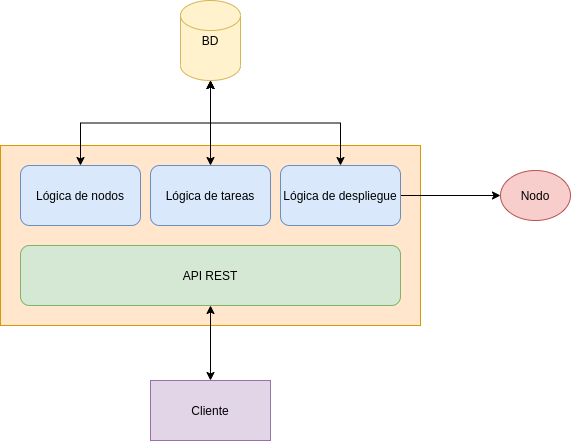
\includegraphics[width=0.8\textwidth]{04-implementation/architecture.png}
    \caption{Diagrama de arquitectura del sistema.}
    \label{fig:04-architecture}
\end{figure}

Volviendo a la figura \ref{fig:04-architecture}, apreciamos que el servidor
también controla el acceso a la base de datos donde se almacena toda la
información sobre los nodos y las tareas. Para esta base de datos, como ya se
indicó en la sección \ref{sec:01-tools}, se ha decidido MongoDB, que es un gestor
de bases de datos documentales y no estructuradas. También se puede comprobar en
el diagrama que el servidor expone todas las funcionalidades del sistema a
través de una API (\textit{Application Programming Interface}). Esta API sigue
el patrón arquitectónico REST (\textit{REpresentation State Transfer}), el cuál
fue introducido en el año 2000 por Roy Fielding en su tesis doctoral
\cite{fielding_architectural_2000}. Simplificando los conceptos que se
desarrollan en esta tesis, podemos identificar las siguientes características
fundamentales del patrón REST:

\begin{itemize}
    \item La interfaz se diseña en torno a recursos, los cuáles son conjuntos de
          información.
    \item Cada recurso está identificado de forma única mediante una URI.
    \item Las operaciones se realizan mediante peticiones HTTP hacia la URI del
          recurso objetivo.
    \item La operación a realizar viene definida por el verbo HTTP usado en la
          petición (\texttt{GET}, \texttt{POST}, \texttt{PUT}, \texttt{PATCH} o
          \texttt{DELETE}).
    \item El servidor no almacena estado alguno, de forma que cada petición debe
          contener toda la información necesaria como para poder darle respuesta.
    \item Para la transferencia de información, se utilizan formatos bien
          definidos como JSON o XML.
\end{itemize}

La aplicación del patrón REST al diseño de interfaces hace que sea más sencillo
estructurar el acceso a la información que contiene un servicio concreto, además
de simplificar también el flujo de trabajo entre cliente y servidor. Para
aplicar REST al diseño de un servicio concreto, se debe identificar cuáles son
los recursos con los que trabaja y qué operaciones permite sobre los mismos. En
el caso de nuestro sistema, tenemos los recursos detallados en las tablas
\ref{tab:04-node_resource} y \ref{tab:04-task_resource}, mientras que las
operaciones posibles se presentan en la sección \ref{sec:server-design}.

\begin{table}[H]
    \centering
    \begin{tabular}{ |>{\columncolor[gray]{0.8}}l|p{0.8\textwidth}| }
        \hline
        Recurso   & Nodo           \\
        \hline
        Atributos &
        \begin{itemize}
            \item ID
            \item Nombre
            \item Dirección IP
            \item Usuario (utilizado para la conexión SSH)
            \item CPU (modelo del procesador)
            \item Arquitectura de CPU (p. ej., \texttt{ARMv7})
            \item Número de núcleos de la CPU
            \item Frecuencia de reloj
            \item RAM
            \item Dispositivos (p. ej., \texttt{/dev/null})
            \item Tareas (que se están ejecutando en el nodo)
        \end{itemize} \\
        \hline
    \end{tabular}
    \caption{Definición del recurso nodo.}
    \label{tab:04-node_resource}
\end{table}

\begin{table}[H]
    \centering
    \begin{tabular}{ |>{\columncolor[gray]{0.8}}l|p{0.8\textwidth}| }
        \hline
        Recurso   & Tarea          \\
        \hline
        Atributos &
        \begin{itemize}
            \item ID
            \item Nombre
            \item Tiempo de ejecución (\textit{runtime})
            \item Límite de tiempo (\textit{deadline})
            \item Período (\textit{period})
            \item Dispositivos (a los que necesita acceder)
            \item Capacidades (p. ej., \texttt{SYS\_NICE})
            \item ID del desplegable (fichero tar con código fuente y \texttt{Dockerfile})
        \end{itemize} \\
        \hline
    \end{tabular}
    \caption{Definición del recurso tarea.}
    \label{tab:04-task_resource}
\end{table}

Como ya se ha indicado, aplicar una arquitectura cliente-servidor como esta
permite reducir al máximo la lógica que contienen los clientes, los cuáles solo
tienen que ocuparse de mostrar la interfaz, comprobar las entradas de los
usuarios y realizar la comunicación con el servidor. Además, el hecho de que el
servidor exponga una API estandarizada facilita enormemente la implementación de
múltiples tipos de aplicaciones cliente, incluso para distintas plataformas (p.
ej., móvil, web o escritorio). Estos clientes sencillamente tienen que consumir
recursos de la interfaz y pueden ofrecer a sus usuarios exactamente las mismas
funcionalidades que los demás. Esta separación de responsabilidades facilita
también el desarrollo y mantenimiento del software, ya que se trata de partes
completamente independientes y separadas que solo deben atenerse a la
especificación de la interfaz mediante la que se conectan.

Por último, también se ha decidido en esta fase de diseño implementar una imagen
Docker, que es el motor de contenedores usado por el sistema, para facilitar el
despliegue de tareas de tiempo real usando el sistema planteado. El
funcionamiento de esta imagen, así como los detalles de diseño e implementación
de las demás partes del sistema, se explican de forma extensiva en las
siguientes secciones de este capítulo. Todo el código desarrollado del que se va
a hablar se encuentra disponible en los repositorios de GitHub del
proyecto\footnote{Repositorio del servidor:
    \url{https://github.com/Varrrro/shipyard-server}}\footnote{Repositorio del
    cliente: \url{https://github.com/Varrrro/shipyard-cli}}\footnote{Repositorio de
    la librería: \url{https://github.com/Varrrro/libshipyard}}.

\section{Servidor maestro}

Tal y como se ha descrito en la sección anterior, el servidor es la parte del
sistema desarrollado que encapsula la lógica principal encargada de llevar a
cabo las funcionalidades deseadas. En esta sección se ahonda en las decisiones
de diseño tomadas para este componente, además de mostrar algunas partes
interesantes de la implementación y las técnicas de prueba e integración
continua aplicadas.

\subsection{Diseño e implementación}
\label{sec:server-design}

A la hora de estructurar el servidor, decidimos hacer una separación por
dominios, de forma que tenemos por un lado la lógica relativa a las
funcionalidades de los nodos y, por otro, la de las tareas. A su vez, también
realizamos una división de responsabilidades, diferenciando entre controladores
y servicios.

Los controladores definen las rutas y operaciones posibles en la API REST del
servidor. Este servidor recibe peticiones HTTP para las rutas que expone, las
cuáles se manejan con distintos controladores dependiendo del verbo HTTP usado.
Estos controladores se encargan entonces de validar los datos recibidos en la
petición, gestionar la autenticación y construir las respuestas con el código de
estado adecuado, llamando a funciones de los servicios para realizar las
operaciones. En los servicios se implementa la lógica encargada de llevar a cabo
estas operaciones como tal, conectando con la base de datos para la gestión de
nodos y tareas, además de llevar a cabo el despliegue de éstas. Como ya se ha
indicado, la lógica se divide también por dominio, de forma que tenemos unos
controladores para las operaciones sobre los nodos y otros separados para las
que ocurren sobre las tareas. Lo mismo ocurre con la lógica de estas operaciones
en los servicios. Para las acciones de orquestación de tareas, además, los
servicios hacen uso de un paquete independiente que implementa estas
funcionalidades concretas. El diagrama de la figura
\ref{fig:04-server_architecture} refleja esta arquitectura que se acaba de
describir.

En cuanto a las operaciones concretas que se pueden realizar mediante la API
REST del servidor, se han definido e implementado las siguientes:

\begin{figure}
    \centering
    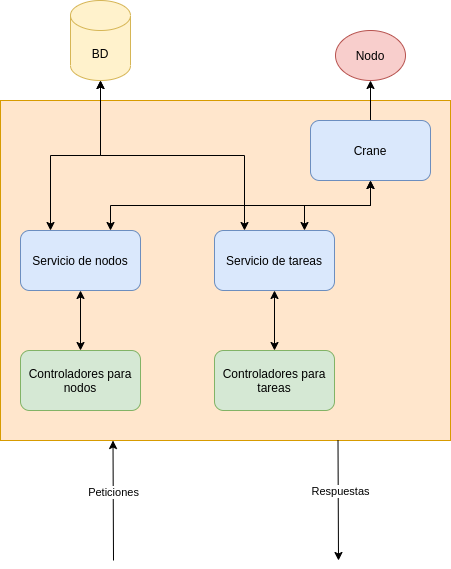
\includegraphics[width=0.9\textwidth]{04-implementation/server.png}
    \caption{Diagrama de arquitectura del servidor.}
    \label{fig:04-server_architecture}
\end{figure}

\begin{itemize}
    \item \texttt{GET /nodes}

          Con esta operación, se obtiene una lista completa de los nodos
          presentes en el sistema. En caso de ocurrir algún error (p. ej., en la
          conexión con la base de datos), el servidor devuelve un una respuesta
          500 (\textit{Internal Server Error}). Si no hay ningún problema, la
          respuesta tiene el código de estado 200 (\textit{Ok}) y contiene en su
          cuerpo la lista de nodos. Cabe destacar que en esta lista de nodos no
          se muestra toda la información presente en la base de datos sobre los
          mismos, sino que se ocultan algunos datos como son el usuario SSH, los
          dispositivos que tiene o los detalles de la CPU.

    \item \texttt{POST /nodes}

          Esta operación permite crear un nuevo nodo, debiendo incluir en el
          cuerpo de la petición los datos del nuevo nodo. No es necesario
          proporcionar valores para todos los atributos definidos en la tabla
          \ref{tab:04-node_resource}, sino que solo son requeridos el nombre,
          dirección IP y número de núcleos de la CPU del nuevo nodo. El nombre
          dado debe ser único, devolviendo el servidor una respuesta 409
          (\textit{Conflict}) si ya está en uso por otro nodo del sistema.

          La petición HTTP que recibe el servidor debe contener en la cabecera
          \textit{Authorization} unas credenciales de autenticación de tipo
          básico, es decir, usuario y contraseña codificados con Base64. Este
          usuario y contraseña son los usados por el servidor para establecer la
          conexión SSH inicial con el nodo. Esta conexión inicial sirve para
          añadir los datos del nodo al fichero \texttt{known\_hosts} del
          servidor con el que se regulan las conexiones SSH conocidas y copiar
          la clave pública de éste al fichero \texttt{authorized\_keys} del
          nodo. Esto permite que las siguientes conexiones SSH que deba realizar
          el servidor usen esta clave para la autenticación, de forma que no sea
          necesario usar la contraseña y aumentando la seguridad.

          Si los datos enviados en el cuerpo de la petición no son correctos, el
          controlador devuelve una respuesta 400 (\textit{Bad Request}). En caso
          de no poder crear el nodo por cualquier otro motivo, se devuelve un
          código 500. La ejecución correcta de esta operación produce una
          respuesta con código de estado 200 y con el nuevo recurso recién
          creado en el cuerpo.

    \item \texttt{GET /nodes?name=<node\_name>}

          Como se puede suponer por el verbo HTTP y la ruta usadas, esta
          operación permite obtener la información detallada de un nodo
          concreto, el cuál se identifica por el nombre proporcionado. Esta
          operación y \texttt{GET /nodes} comparten controlador, comprobándose
          al inicio de éste si en la URI de la petición se encuentra el
          parámetro de consulta \textit{name} para decidir si se llama a la
          función del servicio de nodos que devuelve la lista o a la que
          devuelve los detalles de uno concreto. A diferencia de lo que ocurría
          con esta otra operación, en este caso sí que se devuelven todos los
          atributos del nodo indicado junto con la respuesta 200. Si no se
          encuentra en la base de datos ningún nodo con el nombre indicado, la
          respuesta devuelta tiene un código de estado 404 (\textit{Not Found}).

    \item \texttt{GET /nodes/<node\_id>}

          Esta operación es idéntica a la anterior, siendo la única diferencia
          que la identificación del nodo cuyos detalles se desean obtener se
          realiza por su ID. Esta operación también devuelve una respuesta 200
          con los datos del nodo en el cuerpo en caso de encontrarse en la base
          de datos y un código 404 en caso contrario. También puede devolver una
          raspuesta 409 si el ID dado no es válido, es decir, si no cumple con
          el formato de ID de MongoDB.

    \item \texttt{PUT /nodes/<node\_id>}

          Con esta operación se pueden modificar los atributos de un nodo ya
          existente en el sistema. En el cuerpo de la petición se incluyen solo
          los atributos cuyo valor se desea cambiar junto con estos nuevos
          valores. Si el formato del cuerpo de la petición no es correcto, el
          controlador de la ruta devuelve una respuesta 409. También se devuelve
          este código si el ID indicado no es válido. Si no se encuentra en la
          base de datos del sistema ningún nodo con el ID dado, se devuelve una
          respuesta 404. En caso de realizarse correctamente la operación, la
          respuesta tiene el código de estado 200 y contiene en su cuerpo todos
          los datos del recurso actualizado. Cabe destacar que, si alguno de los
          atributos modificados es el nombre, la IP, el usuario SSH o la lista
          de dispositivos del nodo, el servidor procede a eliminar del mismo
          todas las tareas que tuviera ejecutándose con el fin de evitar
          inconsistencias y estados no recuperables en el sistema. En el
          diagrama de la figura \ref{fig:04-update_node} se refleja este
          comportamiento, además del resto de acciones que lleva a cabo el
          servidor para realizar esta operación.

          \begin{figure}
              \centering
              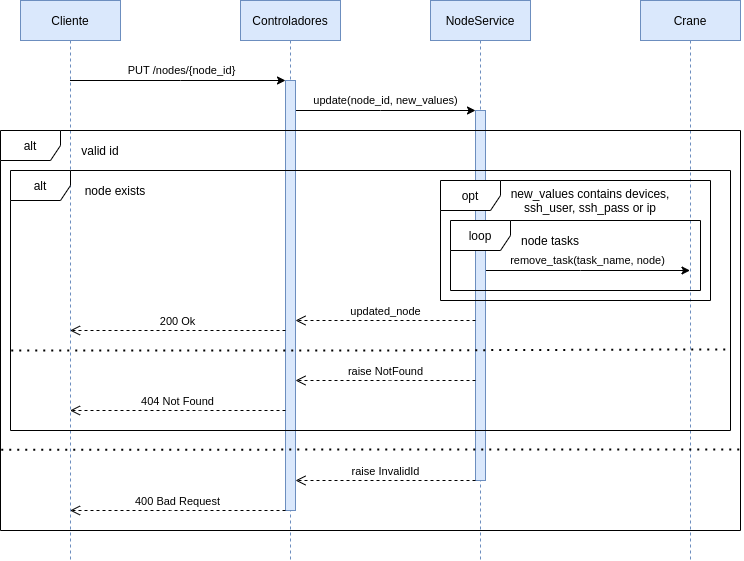
\includegraphics[width=\textwidth]{04-implementation/update-node.png}
              \caption{Diagrama de secuencias de la operación de actualización de un nodo.}
              \label{fig:04-update_node}
          \end{figure}

    \item \texttt{DELETE /nodes/<node\_id>}

          Esta operación permite eliminar un nodo del sistema. Las peticiones no
          necesitan contener ningún dato en el cuerpo, siendo solo necesario
          indicar en la propia ruta de la petición el ID del nodo a eliminar. Si
          este ID no es válido, el controlador devuelve una respuesta 409,
          mientras que si no se encuentra ningún nodo con este ID la respuesta
          es 404. Si la eliminación del recurso se realiza correctamente, la
          respuesta tiene el código de estado 200 y contiene en su cuerpo los
          datos del recurso recién eliminado. Al igual que ocurría con la
          modificación, el sistema se asegura de parar todas las tareas que se
          estuvieran ejecutando sobre el nodo que se elimina y borrarlas del
          mismo, de forma que no queden «restos» en el dispostivo.

    \item \texttt{GET /tasks}

          De forma análoga a la operación \texttt{GET /nodes}, ésta devuelve la
          lista de tareas que están almacenadas en la base de datos del sistema.
          El cuerpo de la respuesta contiene esta lista con el código de estado
          200 si la operación se ha podido realizar correctamente, devolviendo
          el código 500 en caso contrario.

    \item \texttt{POST /tasks}

          Permite añadir una nueva tarea al sistema. A diferencia de las demás
          operaciones, la cabecera \textit{content-type} de las peticiones para
          esta operación, que es la que regula el tipo de contenido, no tiene el
          valor \texttt{application/json}, sino que se usa
          \texttt{multipart/form-data}. Este tipo de contenido se compone de
          múltiples campos, los cuáles pueden ser textuales o archivos, lo cuál
          es necesario para esta operación dado que es necesario aportar tanto
          los metadatos de la tarea en formato JSON como un fichero
          \texttt{tar.gz} con el código fuente y la definición de la imagen
          Docker. El controlador de esta operación se encarga de extraer todos
          estos datos de los dos campos del cuerpo de la petición y, entonces,
          llamar a la función del servicio encargada de realizar la inserción de
          la tarea en la base de datos, devolviendo el controlador una respuesta
          200 si la operación se realiza correctamente. Si el formato de la
          petición recibida es incorrecto (p. ej., falta alguno de los campos),
          se devuelve una respuesta 400. Además, el nombre de la nueva tarea
          debe ser único, obteniendo una respuesta 409 en caso de no serlo. Si
          no se puede crear la tarea por cualquier otra razón, la respuesta
          obtenida es 500.

    \item \texttt{GET /tasks?name=<task\_name>}

          Con esta operación se pueden obtener los detalles de una tarea
          concreta, la cuál se identifica a partir del nombre indicado en el
          parámetro de consulta \textit{name} de la petición. Al igual que
          ocurría con la operación \texttt{GET /nodes?name=<node\_name>}, el
          controlador que da respuesta a esta operación es compartido con el de
          \texttt{GET /tasks}. Al inicio de la ejecución, el controlador
          comprueba la presencia del parámetro \textit{name} en la petición,
          devolviendo los detalles de la tarea o la lista completa de tareas
          según si está presente o no. En caso de operación correcta, la
          respuesta 200 incluye en el cuerpo los datos del recurso deseado a
          excepción del fichero \texttt{tar.gz} con su código fuente. Si este
          recurso no se encuentra, el código devuelto es 404, devolviendo 500 en
          cualquier otro caso.

    \item \texttt{GET /tasks/<task\_id>}

          Al igual que la operación anterior, ésta también devuelve los detalles
          de una tarea, aunque en este caso se usa el ID de la misma para su
          identificación. Si este ID no es válido, el controlador devuelve una
          respuesta 400; mientras que si no se encuentra en la base de datos
          ninguna tarea con este ID, la respuesta es 404. Esta operación tampoco
          devuelve el fichero de despliegue asociado a la tarea. Si no se puede
          realizar la operación, el controlador devuelve una respuesta 500.

    \item \texttt{PUT /tasks/<task\_id>}

          Modificación de una tarea. Como ocurría en la operación de creación de
          tareas, las peticiones también tienen el tipo de contenido
          \texttt{multipart/form-data}. Como diferencia, no es necesario que la
          petición contenga tanto el dichero \texttt{tar.gz} con el código
          fuente como el JSON con los atributos, sino que solo debe contener lo
          que se vaya a actualizar. Antes de modificar la tarea, el servidor se
          asegura de eliminarla de cualquier nodo en el que se estuviera
          ejecutando para evitar inconsistencias en el sistema. Si el ID dado o
          el formato del cuerpo de la petición no son válidos, el controlador
          devuelve una respuesta 400. Si no se encuentra en la base de datos
          ninguna tarea con el ID indicado, se devuelve un 404. En caso de
          realizarse la operación correctamente, la respuesta devuelta tiene el
          código 200 y contiene en su cuerpo el recurso actualizado. Si no se
          puede realizar la operación por cualquier otra razón, devuelve una
          respuesta 500.

    \item \texttt{DELETE /tasks/<task\_id>}

          Elimina una tarea de la base de datos del sistema, identificada por el
          ID indicado en la propia petición. Si no se encuentra ninguna tarea
          con dicho ID, devuelve 404. Si este ID no es válido, devuelve 400. Si
          no se puede realizar la operación por cualquier otra razón, devuelve
          500. Cuando la eliminación se completa de forma satisfactoria, el
          controlador devuelve una respuesta con código 200 y con el recurso
          recién eliminado en el cuerpo.

    \item \texttt{POST /nodes/<node\_id>/tasks?task\_id=<task\_id>}

          Esta operación permite el despliegue de una tarea dada en un nodo. Es,
          quizás, la operación más compleja que realiza el servidor. Se recibe
          una petición en cuya ruta se se encuentra el ID del nodo, aportándose
          el de la tarea como un parámetro de consulta (\textit{query}). Si este
          parámetro de consulta no está presente en la petición, el controlador
          devuelve inmediatamente una respuesta 400. Si todos los valores están
          presentes, se llama entonces a la función del servicio encargada de
          llevar a cabo el despliegue.

          Esta función convierte los IDs a los propios de MongoDB, lanzando un
          error \texttt{InvalidId} en caso de que su formato no sea correcto. El
          controlador devolvería entonces una respuesta 400 al cliente. El
          servicio puede devolver un error \texttt{NotFound} si no encuentra en
          la base de datos los recursos deseados, error que captura el
          controlador para generar una respuesta 404. Si los IDs se corresponden
          con recursos existentes en el sistema, el servicio procede a comprobar
          que el nodo posea todos los dispositivos que necesita la tarea. Si no
          es así, el servicio lanza un error \texttt{MissingDevices} que es
          capturado por el controlador, que genera una respuesta 500. La última
          comprobación que se realiza es la de la viabilidad de la ejecución del
          conjunto de tareas que se obtendría al añadir la nueva tarea a las que
          ya se están ejecutando en el nodo. Tanto para realizar esta
          comprobación como para llevar a cabo el despliegue como tal, el
          servicio se apoya en el paquete interno \textit{crane} que ya fue
          introducido al inicio de esta sección. La función
          \texttt{check\_feasibility} de este paquete es comprueba esta
          viabilidad. Esta función recibe el conjunto de tareas y el número de
          núcleos de la CPU del nodo objetivo. Con estos datos, se calcula la
          utilización de CPU para determinar si la ejecución es viable o no
          \cite{zhang_schedulability_2009}. Cabe destacar que, si el nodo tiene
          más de un núcleo (multiprocesador), esta comprobación de la
          utilización no es condición suficiente para asegurar la viabilidad del
          conjunto de tareas, aunque en esta primera versión de la herramienta
          no se gestiona esta situación.

          \begin{figure}
              \centering
              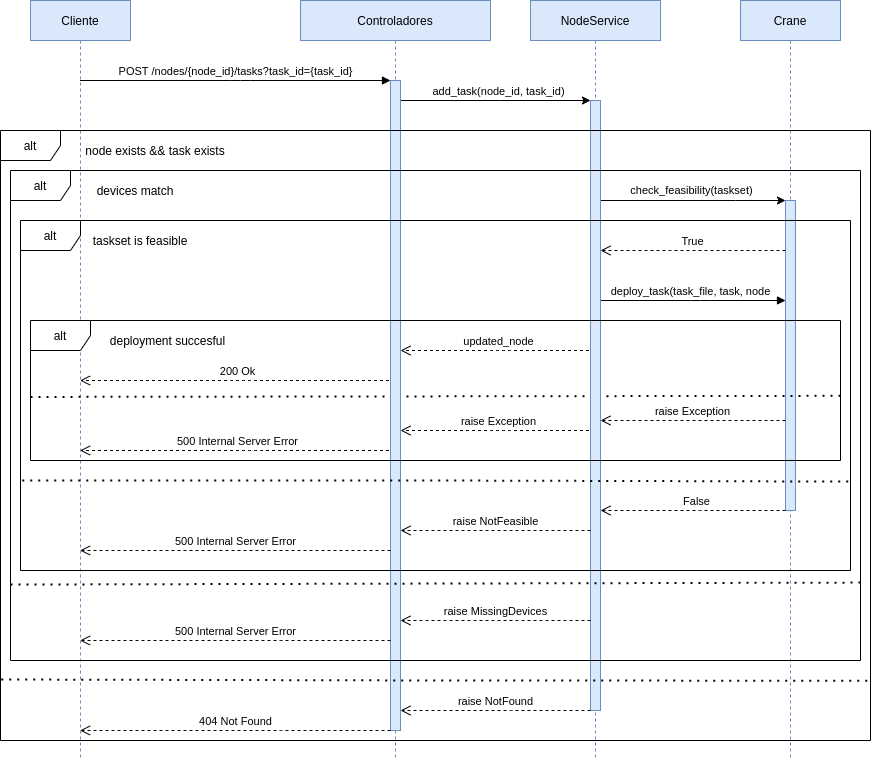
\includegraphics[width=\textwidth]{04-implementation/deploy-task.png}
              \caption{Diagrama de secuencias de la operación de despliegue de una tarea.}
              \label{fig:04-deploy_task}
          \end{figure}

          Si la función \texttt{check\_feasibility} determina que el conjunto de
          tareas es viable, entonces se ejecuta otra función del paquete
          \textit{crane} para realizar el despliegue: \texttt{deploy\_task}.
          Esta función recibe como entrada el fichero \texttt{tar.gz} de la
          tarea, así como sus metadatos y los del nodo. Con estos datos, se
          establece una conexión con el demonio Docker del nodo mediante SSH,
          obteniendo un cliente con el que se construye la imagen a partir del
          fichero \texttt{tar.gz} y se lanza el contenedor. Los parámetros de
          planificación de la tarea (tiempo de ejecución, límite de tiempo y
          período) se le pasan al contenedor como variables de entorno, las
          cuáles luego usará la librería para fijar la planificación.

          Cualquier tipo de excepción que se lance durante este despliegue será
          capturada por el controlador para generar una respuesta 500. Si la
          operación se realiza correctamente, el servidor responde con una
          respuesta 200 que contiene en su cuerpo los detalles del nodo
          actualizado, incluyendo ya en su lista de tareas la que se acaba de
          añadir. Todo este proceso que se acaba de describir para realizar la
          operación de despliegue se puede observar de manera esquematizada en
          el diagrama de secuencias de la figura \ref{fig:04-deploy_task}.

    \item \texttt{DELETE /nodes/<node\_id>/tasks/<task\_id>}

          Esta operación permite parar la ejecución de una tarea desplegada en
          un nodo concreto, elmininándola del mismo. Las peticiones recibidas
          para esta operación contienen en la ruta los valores de los IDs del
          nodo y la tarea en cuestión. El controlador entonces llama a la
          función del servicio encargada de realizar la operación.

          Lo primero que hace el servicio es comprobar si están presentes en la
          base de datos algunos recursos con los IDs proporcionados, lanzando un
          error \texttt{NotFound} en caso de no encontrarlos. Este error es
          entonces capturado por el controlador, que genera una respuesta 404
          para el cliente. Si al buscar los recursos en la base de datos resulta
          que los IDs no son válidos, se lanza un error \texttt{InvalidId}, para
          el que el controlador crea una respuesta 400.

          Si los recursos existen, el servicio entonces ejecuta la función
          \texttt{remove\_task} del paquete \textit{crane} para que se lleve a
          cabo la eliminación. Al igual que ocurría en la de despliegue de
          tareas, se crea un cliente para el servidor Docker del nodo mediante
          SSH usando las claves almacenadas. A través de este cliente, se
          elimina el contenedor en el que se ejecuta la tarea y, también, la
          imagen asociada. Una vez termina esta operación, se actualiza la base
          de datos para quitar la tarea de la lista que tiene asociada el nodo.
          Si durante la eliminación ocurre algún error, el controlador la
          captura y devuelve una respuesta 500 al cliente. Si la operación se
          realiza correctamente, la respuesta tiene un código de estado 200 y
          contiene en su cuerpo los datos actualizados del nodo, ya sin la tarea
          en su lista de tareas.
\end{itemize}

Gracias al uso de la librería \textit{hug}, la implementación de los
controladores es extremadamente sencilla. Cada controlador es una simple función
Python que, mediante decoradores, se enlaza con una operación concreta del
servidor a la que da respuesta. En el listado \ref{lst:04-post_node_tasks}, se
presenta el controlador de la operación de despligue de tareas. Como se puede
observar, es con el decorador \lstinline{@hug.post} con el que indicamos que se
debe ejecutar esta función cuando se reciba una petición POST para la ruta
\texttt{/nodes/<node\_id/tasks}\footnote{La ruta \texttt{/nodes} es la base para
    todos los controladores de los nodos, por eso no se muestra en el decorador.}.
Se definen aquí también las variables de ruta presentes, que en este caso es el
ID del nodo.

\begin{lstlisting}[
    language=Python,
    caption={Controlador de la operación de despliegue de tareas.},
    label={lst:04-post_node_tasks},
    showstringspaces=false
]
@hug.post('/{node_id}/tasks')
def post_node_tasks(node_id: str, response, task_id: str = None):
    if task_id is None:
        response.status = hug.HTTP_BAD_REQUEST
        return {
            'error': 'No task ID was specified in the request'
        }

    try:
        result = NodeService.add_task(node_id, task_id)
        if result is None:
            response.status = hug.HTTP_INTERNAL_SERVER_ERROR
            return {'error': 'Unable to add task to node.'}
        return Node.Schema().dump(result)
    except InvalidId as e:
        response.status = hug.HTTP_BAD_REQUEST
        return {'error': str(e)}
    except NotFound as e:
        response.status = hug.HTTP_NOT_FOUND
        return {'error': str(e)}
    except (NotFeasible, MissingDevices) as e:
        response.status = hug.HTTP_INTERNAL_SERVER_ERROR
        return {'error': str(e)}
    except Exception:
        response.status = hug.HTTP_INTERNAL_SERVER_ERROR
        return {'error': 'Unable to add task to node.'}   
\end{lstlisting}

Las funciones definidas como controladores con \textit{hug} reciben
estas variables de ruta como argumentos, teniendo también los posibles
parámetros de consulta (\texttt{task\_id}) y los objetos propios de la
comunicación HTTP (p. ej., \texttt{request}, \texttt{response}, \texttt{body}).
Observando el listado, se aprecia claramente cómo los controladores se encargan
solo de comprobar que el formato de la petición sea el correcto, llamar a la
función del servicio apropiada para realizar la operación y construir la
respuesta que corresponda en base al resultado de la misma, tal y como se
describía anteriormente.

\begin{lstlisting}[
    language=Python,
    caption={Función del servicio de tareas para la creación de tareas.},
    label={lst:04-task_service_create},
    showstringspaces=false
]
@staticmethod
def create(
    new_task: Task,
    file_name: str,
    file_body: BytesIO
    ) -> str:

    result = db.tasks.find_one({'name': new_task.name})
    if result is not None:
        raise AlreadyPresent(
            'A task already exists with the given name.'
        )

    file_id = fs.put(file_body, filename=file_name)
    new_task.file_id = file_id

    new_id = db.tasks.insert_one(Task.Schema(
        exclude=['_id']).dump(new_task)).inserted_id
    return str(new_id)
\end{lstlisting}

Por otro lado, en el listado \ref{lst:04-task_service_create} se muestra la
función del servicio de tareas que implementa la lógica encargada de la creación
de éstas. El objeto \texttt{db}, como se puede suponer, es la conexión con la
base de datos que mantiene el servidor. Esta función concreta tiene una
particularidad con respecto a las demás: se debe almacenar también el fichero
\texttt{tar.gz} con el código fuente y la definición de imagen de la tarea. Para
ello, usamos GridFS, que es la especificación de MongoDB para el almacenamiento
de ficheros de gran tamaño. De esta forma, se pueden almacenar los ficheros en
colecciones normales de MongoDB sin necesitar de otro tipo de almacenamiento. Al
igual que el objeto \texttt{db} era la conexión con la base de datos MongoDB,
\texttt{fs} es la conexión con la parte de GridFS. Entonces, para añadir una
nueva tarea al sistema, primero se añade el fichero con \texttt{fs.put()} y, con
el ID recién obtenido para el mismo, se crea el nuevo documento en la colección
de tareas.

Otro aspecto a destacar es el uso de \texttt{BytesIO} para el acceso al fichero.
Cuando el controlador de la operación \texttt{POST /tasks} recibe una nueva
petición, extrae el contenido del fichero del cuerpo de la misma y lo escribe a
un objeto de este tipo. A todos los efectos, un objeto \texttt{BytesIO} actúa
como un archivo normal, con la diferencia de que sus datos se almacenan
directamente en memoria en vez de en el sistema de archivos. Al usar este
mecanismo, conseguimos hacer que el proceso de inserción de la tarea sea más
rápido, dado que no tenemos que acceder a disco duro ni tenemos que trabajar con
ficheros.

Como se ha indicado en la sección \ref{sec:04-system_design}, la API REST usa el
formato estándar de codificación de datos JSON para la transmisión de
información entre el servidor y los clientes. La mayoría de las peticiones y
respuetas contienen en sus cuerpos una representación de los recursos del
sistema en este formato. Para que la serialización de los objetos Python a JSON
y viceversa se realice de forma más sencilla, se ha usado la librería
\textit{marshmallow}. Esta librería nos permite definir esquemas de datos para
los recursos del sistema que, además de ayudar con la serialización y
deserialización, proporciona un mecanismo de validación automática sobre los
datos recibidos de los clientes.

\subsection{Prueba}

Para asegurar el correcto funcionamiento del código implementado, se han escrito
pruebas unitarias. Este tipo de pruebas se centran en validar el comportamiento
de partes individuales del sistema, aíslandolas del resto. En nuestro caso, las
pruebas se realizan para las funciones de los controladores y los servicios. La
librería \textit{unittest}, que forma parte de la librería estándar de Python,
proporciona los mecanismos que se han utilizado para implementar estas pruebas.
Con esta librería, se definen clases \texttt{TestCase}, que son las unidades
individuales de prueba para un componente concreto. Las funciones de estas
clases son las que comprueban que las salidas obtenidas para determinadas
entradas son las correctas en las funciones individuales del componente dado.
Para nuestro servidor, se han definido cuatro clases \texttt{TestCase} para los
cuatro componentes principales: controladores de los nodos, controladores de las
tareas, servicio de nodos y servicio de tareas.

\begin{lstlisting}[
    language=Python,
    caption={Prueba unitaria del controlador para el despliegue de tareas.},
    label={lst:04-post_node_tasks_test}
]
def test_post_node_tasks(self):
    response = hug.test.call(
        'POST', controllers, f'{test_nodes[0]._id}/tasks',
        params={
            'task_id': 'Test'
    })
    self.assertEqual(response.status, hug.HTTP_OK)
    self.assertIsNotNone(response.data)

    response = hug.test.call(
        'POST', controllers, f'{ObjectId()}/tasks', params={
            'task_id': 'Test'
    })
    self.assertEqual(response.status, hug.HTTP_NOT_FOUND)
    self.assertIsNotNone(response.data)
    self.assertIsInstance(response.data['error'], str)

    response = hug.test.call(
        'POST', controllers, f'{test_nodes[0]._id}/tasks')
    self.assertEqual(response.status, hug.HTTP_BAD_REQUEST)
    self.assertIsNotNone(response.data)
    self.assertIsInstance(response.data['error'], str)

    response = hug.test.call(
        'POST', controllers, f'error/tasks', params={
            'task_id': 'Test'
    })
    self.assertEqual(response.status, hug.HTTP_BAD_REQUEST)
    self.assertIsNotNone(response.data)
    self.assertIsInstance(response.data['error'], str)

    response = hug.test.call(
        'POST', controllers, f'{test_nodes[0]._id}/tasks',
        params={
            'task_id': 'MissingDevices'
    })
    self.assertEqual(
        response.status, hug.HTTP_INTERNAL_SERVER_ERROR)
    self.assertIsNotNone(response.data)
    self.assertIsInstance(response.data['error'], str)

    response = hug.test.call(
        'POST', controllers, f'{test_nodes[0]._id}/tasks',
        params={
            'task_id': 'NotFeasible'
    })
    self.assertEqual(
        response.status, hug.HTTP_INTERNAL_SERVER_ERROR)
    self.assertIsNotNone(response.data)
    self.assertIsInstance(response.data['error'], str)
\end{lstlisting}

Como se acaba de explicar, una prueba unitaria valida una única parte del código
de forma aislada. En nuestro servidor, tanto los servicios como los
controladores deben interactuar con otros componentes para cumplir su función.
Para poder probar solo una función concreta, necesitamos hacer maquetas o
\textit{mocks} de los demás componentes con los que interactúa. Estas maquetas
son implementaciones de prueba, en muchos casos vacías o con un comportamiento
concreto para cada caso de prueba. Por ejemplo, para poder probar los
controladores, necesitamos una maqueta del servicio con el que trabajan. La
maqueta ofrece una implementación «de juguete» con un comportamiento igual al
que tendría el servicio real. La librería \textit{unittest} proporciona el
decorador \texttt{@mock.patch} para las clases \texttt{TestCase}, con el cuál se
puede proporcionar una maqueta para que sea usada por el código que se prueba en
lugar del elemento real.

En el listado \ref{lst:04-post_node_tasks_test} se puede ver la función de
prueba para el controlador de despliegue de tareas del \texttt{TestCase} de los
controladores de los nodos. En \ref{lst:04-post_node_tasks} se puede ver como
este controlador llama a la función \texttt{add\_task} del servicio de nodos. La
maqueta del servicio que se usa para esta prueba tiene una implementación simple
de esta función que, dependiendo de la entrada dada, permite obtener todas los
resultados que se podrían obtener con la implementación real. De esta forma,
podemos comprobar que el controlador se comporte correctamente para cada una de
estas salidas.

Volviendo a la prueba de \ref{lst:04-post_node_tasks_test}, consiste
sencillamente de una serie de peticiones con distintos valores que se envían al
controlador gracias a la función \texttt{hug.test.call()} que la propia librería
\textit{hug} proporciona para escribir pruebas. Para cada petición, se comprueba
que la respuesta tiene el código de estado HTTP correcto, además de los valores
deseados en el cuerpo.

\begin{lstlisting}[
    language=Python,
    caption={Prueba unitaria de la función de creación de tareas.},
    label={lst:04-task_service_create_test}
]
def test_create(self):
    new_task = Task.Schema().load({
        'name': 'Test',
        'runtime': 1000,
        'deadline': 1000,
        'period': 1000
    })

    try:
        result = TaskService.create(
            new_task, 'test_file.tar.gz', BytesIO())
        self.assertEqual(
            mockdb.tasks.count_documents({}), len(test_tasks)+1)
        self.assertIsInstance(result, str)
    except:
        self.fail()

    with self.assertRaises(AlreadyPresent):
        TaskService.create(
            new_task, 'test_file.tar.gz', BytesIO())
    self.assertEqual(
        mockdb.tasks.count_documents({}), len(test_tasks)+1)
\end{lstlisting}

Los servicios, por otro lado, interactúan tanto con la base de datos MongoDB
como con las funciones de la librería interna \textit{crane}. Estas funciones se
pueden maquetar al igual que hacíamos con las de los propios servicios para
probar los controladores dado que conocemos su implementación y su alcance es
pequeño. La conexión con la base de datos plantea una situación diferente.
Podríamos levantar una instancia de MongoDB cada vez que quisiéramos ejecutar
las pruebas, aunque esto rompe ligeramente con el enfoque aislado de las pruebas
unitarias. Además, esto tiene un impacto considerable en la complejidad de la
ejecución de estas pruebas, que deberían ser simples y directas. Por ello,
hacemos uso de la librería \textit{mongomock}, que nos proporciona una maqueta
de los clientes de MongoDB usados por los servicios. Estas maquetas funcionan
exactamente igual que los clientes normales, almacenando los datos de la
hipotética base de datos en memoria y permitiendo comprobar que las operaciones
se realizan correctamente. Antes de ejecutar las pruebas de los servicios, se
añaden datos de prueba a estas maquetas, de forma que se simule una base de
datos real en producción.

Por lo demás, las pruebas como tal son muy similares a las de los controladores,
tal y como se puede ver en el listado \ref{lst:04-task_service_create_test}. En
él, se muestra la validación del funcionamiento de la lógica de creación de
tareas que fue expuesta en \ref{lst:04-task_service_create}, que consiste en
añadir una tarea simple y comprobar que en la base de datos maquetada
(\texttt{mockdb}) se ha añadido el nuevo documento. Se repite la inserción para
asegurar que no se pueden crear elementos duplicados.

\subsection{Integración continua}

Para facilitar el despliegue de este servidor en múltiples plataformas, se ha
definido una imagen Docker sencilla. Esta imagen se puede encontrar en el
repositorio de DockerHub\footnote{Enlace a la imagen:
    \url{https://hub.docker.com/repository/docker/varrrro/shipyard-server}}. La
construcción de la imagen se realiza de forma automática cuando se publica una
nueva versión del servidor en el repositorio de GitHub del mismo gracias a
GitHub Actions. Esta funcionalidad de GitHub permite definir secuencias de pasos
que se ejecutan cuando ocurren ciertos eventos en el repositorio.

Además de construir la imagen y publicarla en DockerHub para cada nueva
\textit{release}, se ha definido otra acción que ejecuta las pruebas unitarias
del proyecto de forma automática para cada nuevo cambio que se realiza sobre la
base de código del repositorio. Al ejecutar las pruebas, se obtiene además un
informe de la cobertura del código que se envía a Codecov. La cobertura mide el
porcentaje de líneas de código del proyecto que son ejecutadas por alguna
prueba. Codecov permite visualizar estos informes de manera sencilla con paneles
de control como el mostrado en la figura \ref{fig:01-codecov}. De esta forma,
podemos monitorizar la calidad del código y comprobar si los nuevos cambios
introducidos siguen pasando las pruebas de forma correcta.

\section{Cliente de terminal}

El diseño detallado en la sección \ref{sec:04-system_design} especificaba que
todas las funcionalidades del sistema se recogen en un servidor maestro que
expone las distintas operaciones a través de una API REST. Este modelo
cliente-servidor permite la implementación de múltiples clientes para
plataformas diferentes de forma sencilla. En nuestro caso, se ha decidido
acompañar esta primera versión del sistema con un cliente de línea de comandos
que permita llevar a cabo las distintas operaciones existentes.

Aunque un cliente con interfaz gráfica es más accesible y fácil de usar, se ha
decidido hacerlo de terminal debido a que es más versátil: fácilmente se puede
incorporar en \textit{scripts} de \texttt{bash} y tareas automáticas de
\texttt{cron}, además de ser usado con herramientas de integración continua
modernas.

\subsection{Diseño e implementación}

De forma idéntica a como sucedía con el servidor, la lógica del cliente se ha
dividido por dominio y responsabilidades. En este caso, la división por dominio
se realiza en tres partes: operaciones de nodos, de tareas y de orquestación.
Para cada uno de estos dominios, tenemos dos componentes separados: los comandos
y los servicios. Los primeros, como su propio nombre indica, definen los
comandos que puede ejecutar el usuario desde la terminal, indicando todos los
argumentes necesarios y las opciones disponibles. Los comandos validan la
información introducida por el usuario, llamando después a los servicios para
llevar a cabo las operaciones. Estos servicios son, al igual que ocurría con el
servidor, clases con métodos estáticos que implementan la lógica de negocio de
la aplicación. En el cliente, los servicios se encargan de realizar las
peticiones HTTP al servidor y procesar las respuestas. Según la respuesta
recibida, las funciones de los servicios pueden devolver los datos esperados o
lanzar errores, en base a los cuáles el comando mostrará una respuesta u otra en
la terminal para el usuario.

A continuación, se presentan y detallan todos los comandos que se han definido
para esta primera versión del cliente. Todas las operaciones comienzan con el
comando base \texttt{shipyard}, que es el nombre que se le ha dado al sistema.

\begin{itemize}
    \item \lstinline{shipyard node ls}

          Con este comando, se obtiene del servidor una lista con todos los nodos
          presentes en el sistema. El cliente imprime en la terminal una tabla con
          el ID, nombre, dirección IP y número de tareas en ejecución de cada
          nodo.

          Si se usa la opción \texttt{--active}, solo se muestran aquellos nodos
          en los que se está ejecutando al menos una tarea.

    \item \lstinline{shipyard node inspect <key>}

          En este caso, se buscan los detalles de un nodo concreto, identificado
          por la clave dada. Esta clave puede ser tanto el ID del nodo como su
          nombre. Es la función del comando la encargada de comprobar si se trata
          de un ID válido  para llamar a la función \lstinline{get_by_id} del
          servicio, llamando a \lstinline{get_by_name} si no lo es.

          El comando imprime en la terminal es su lista de tareas, mostrando el
          ID, nombre, tiempo de ejecución (\textit{runtime}), límite de tiempo
          (\textit{deadline}), período (\textit{period}) de cada una de ellas. Si
          el servidor responde con un error (p. ej., si no se encuentra ningún
          nodo con la clave dada), se indica al usuario.

    \item \lstinline{shipyard node add <name> <address> <cpu-cores>}

          Con este comando, el usuario puede añadir un nuevo nodo al sistema. En
          la ejecución del propio comando, se indican el nombre, la dirección IP y
          el número de núcleos del CPU del nuevo nodo. Inmediatamente después de
          introducir el comando en la terminal, la aplicación pide al usuario que
          introduzca el nombre de usuario y la contraseña para realizar la
          conexión SSH inicial con el dispositivo y copiar las claves.

          Si el usuario desea especificar más valores para otros atributos del
          nodo, puede usar las opciones disponibles para el comando:
          \texttt{--cpu}, \texttt{--cpu-arch}, \texttt{--cpu-freq}, \texttt{--ram}
          y \texttt{--device}.

          En pantalla se imprime el ID del nuevo nodo si la operación se ha
          realizado correctamente, de forma que el usuario pueda realizar más
          operaciones con él. Si la respuesta del servidor no es correcta, se
          imprime el mensaje de error adecuado por la terminal para informar al
          usuario.

    \item \lstinline{shipyard node update <key> <values>}

          Este comando se puede usar para cambiar los atributos de un nodo ya
          presente en el sistema. Al igual que ocurría con el comando
          \lstinline{node inspect}, el nodo se puede identificar tanto por su ID
          como por su nombre. El argumento \textit{values} del comando debe ser
          una cadena de texto en formato JSON con los pares clave-valor de los
          atributos a actualizar. Si el formato de la cadena proporcionada no es
          correcto, se imprime un mensaje de error para el usuario y la operación
          se cancela. En caso de ser correcto, se llama a la función del servicio
          encargada de realizar la petición de modificación.

          Se debe tener en cuenta que, si el nombre del nodo o su lista de
          dispositivos son modificados, realizar esta operación conlleva la
          suspensión de la ejecución de todas las tareas que hubiera en dicho
          nodo. Tanto si la operación se realiza correctamente como si no, se
          muestra un mensaje en la terminal para informar al usuario del
          resultado.

    \item \lstinline{shipyard node rm <key>}

          Un usuario puede eliminar un nodo usando este comando. Una vez más, se
          puede identificar el nodo a eliminar tanto por su ID como por su nombre.
          Al ejecutar este comando, el usuario debe confirmar que desea realizar
          la operación para evitar accidentes. Al terminar la operación, se
          muestra un mensaje por la terminar para informar al usuario del
          resultado.

    \item \lstinline{shipyard task ls}

          Al igual que el comando \lstinline{node ls}, este comando sirve para
          obtener una lista de las tareas almacenadas en el sistema. Se imprime en
          la pantalla una tabla que muestra el ID, nombre, tiempo de ejecución,
          límite de tiempo y período de cada tarea.

    \item \lstinline{shipyard task add <name> <runtime> <deadline> <period> <file>}

          Este comando es el usado para añadir una nueva tarea al sistema. En los
          argumentos, se indican los valores necesarios para la tarea: nombre,
          tiempo de ejecución, límite de tiempo, período y el fichero
          \texttt{tar.gz} que contiene los desplegables de la tarea. Si el usuario
          desea especificar también una serie de dispositivos que necesita la
          tarea, puede hacerlo con la opción \texttt{--device} e indicar tantos
          como quiera. Si la operación se realiza correctamente, el ID de la nueva
          tarea se imprime por la terminal. Por el contrario, si ocurre algún
          error que impida la realización de la operación, se informa al
          usuario.

          \begin{figure}
              \centering
              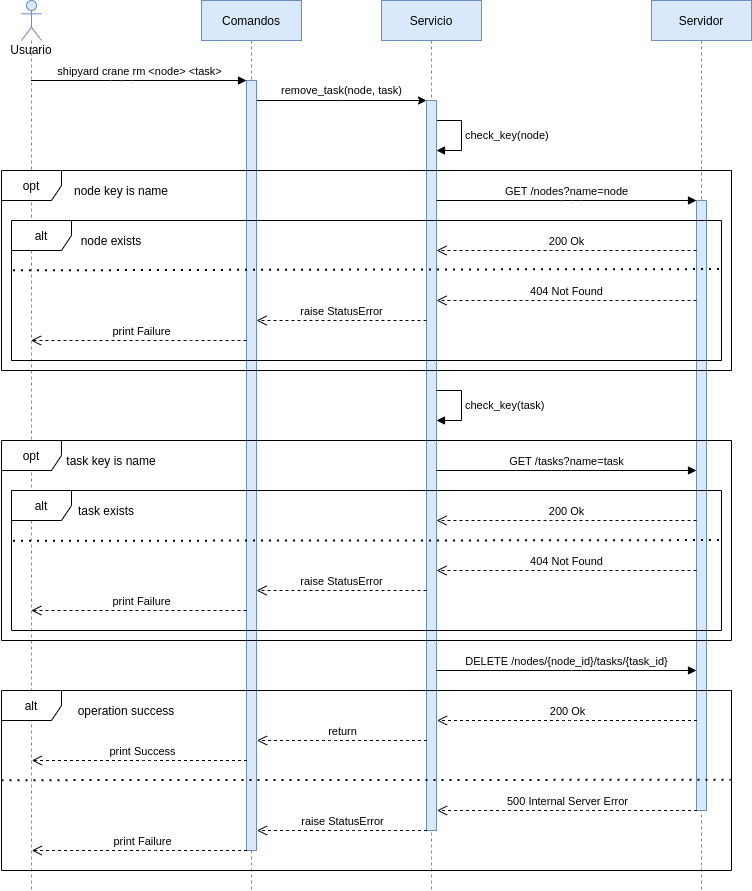
\includegraphics[width=\textwidth]{04-implementation/cli-remove-task-node.png}
              \caption{Diagrama de secuencias del comando de de eliminación de una tarea de un nodo.}
              \label{fig:04-cli_remove_task_node}
          \end{figure}

    \item \lstinline{shipyard task update <key> <values>}

          Un usuario puede actualizar una tarea usando este comando. Al igual que
          ocurría con el comando \lstinline{node update}, se pasan como argumentos
          la clave que identifica la tarea que se debe actualizar y los nuevos
          valores de los atributos en formato JSON. La clave puede ser tanto el ID
          de la tarea como su nombre. Si el usuario desea actualizar también el
          fichero \texttt{tar.gz} asociado a la tarea, debe usar la opción
          \texttt{--file} junto con la ruta del nuevo fichero.

          Tanto si la operación se realiza correctamente como si no, se imprime
          por pantalla un mensaje para informar al usuario del resultado. Cabe
          destacar que la operación del servidor a la que se llama para actualizar
          una tarea provoca la eliminación de dicha tarea de todos los nodos en
          los que se estuviera ejecutando.

    \item \lstinline{shipyard task rm <key>}

          Con este comando, el usuario puede eliminar una tarea del sistema. El
          argumento \textit{key} es la clave con la que se identifica la tarea a
          eliminar, ya sea su ID o su nombre. Al eliminar una tarea, la operación
          del servidor a la que se llama se encarga de eliminarla de todos los
          nodos en los que se estuviera ejecutando. Tanto si la operación se
          realiza correctamente como si no, se imprime por pantalla un mensaje
          para informar al usuario del resultado.

    \item \lstinline{shipyard crane deploy <node-key> <task-key>}

          Esta es, quizás, la operación más importante que se puede realizar desde
          el cliente. Permite a un usuario desplegar una tarea del sistema en un
          nodo concreto. El nodo y la tarea en cuestión se identifican por las
          claves pasadas como argumentos del comando. Estas claves pueden ser
          tanto sus IDs como sus nombres. La función del comando entonces llama a
          la función del servicio \textit{crane} encargada de enviar la petición
          HTTP al servidor para que se realice la operación. Se informa al usuario
          del resultado de la operación mediante un mensaje que se imprime en la
          terminal.

    \item \lstinline{shipyard crane rm <node-key> <task-key>}

          Al igual que el usuario puede desplegar tareas en los nodos, también
          puede retirarlas de estos usando este comando. De nuevo, el nodo y la
          tarea concretos son identificados por las claves pasadas como argumentos
          en la llamada al comando y pueden ser tanto sus IDs como sus nombres.
          Después, la función del servicio \textit{crane} se encarga de realizar
          la petición HTTP apropiada y procesar la respuesta, informando el
          comando al usuario del resultado mediante un mensaje impreso en la
          terminal. En la figura \ref{fig:04-cli_remove_task_node} se muestra en
          un diagrama de secuencias la lógica de ejecución de este comando.

    \item \lstinline{shipyard config <key> <value>}

          Este comando permite cambiar la configuración de la aplicación. Se
          debe indicar en los argumentos el parámetro a cambiar (\textit{key}) y
          el nuevo valor (\textit{value}). Se usa principalmente para
          especificar la dirección del servidor maestro.
\end{itemize}

Definir los comandos es relativamente sencillo gracias a la librería
\textit{click}. Sencillamente, definimos una función Python para cada comando y
usamos decoradores para indicar que es un comando y definir los argumentos y
opciones, de forma similar a lo que hacíamos con \textit{hug} para definir los
controladores de la API REST del servidor. En el listado de código
\ref{lst:04-cli_task_add_command} se muestra la función implementada para el
comando \texttt{shipyard task add}. Vamos a explicar qué significa cada
decorador usado:

\begin{itemize}
    \item \texttt{@task.command}: Normalmente, se usa el decorador
          \texttt{@click.command} para indicar que una función es un comando de la
          aplicación. Aquí, se usa \texttt{task} debido a que es un subcomando del
          comando base con el mismo nombre.
    \item \texttt{@click.pass\_obj}: Usado para pasar el contexto de la
          aplicación, que contiene el servicio apropiado (en este caso, el de tareas),
          a la función.
    \item \texttt{@click.option}: Son las opciones no requeridas que se pueden
          indicar en la ejecución del comando. Pueden ser de cualquier tipo y, como
          ocurre en el ejemplo mostrado, de uso múltiple.
    \item \texttt{@click.argument}: Los argumentos obligatorios del comando.
          Pueden ser de cualquier tipo.
\end{itemize}

Como se puede apreciar en el listado; el contexto, las opciones y los argumentos
son también argumentos de la función. Entrando ya en la implementación de la
operación como tal, se puede ver como se crea el objeto \texttt{Task} con los
datos dados usando un esquema definido con la librería \textit{marshmallow}.
Igual que ocurría en el servidor, usamos esta librería para facilitar el trabajo
con los recursos, haciendo muy sencillo el paso de objeto Python a diccionario y
viceversa.

\begin{lstlisting}[
    language=Python,
    caption={Comando para la creación de una nueva tarea.},
    label={lst:04-cli_task_add_command},
    showstringspaces=false
]
@task.command()
@click.pass_obj
@click.option(
    '--device', type=str, multiple=True,
    help='A device needed for the task.'
)
@click.argument('name', type=str)
@click.argument('runtime', type=int)
@click.argument('deadline', type=int)
@click.argument('period', type=int)
@click.argument('file', type=click.File('rb'))
def add(service, device, name, runtime, deadline, period, file):
    try:
        task = Task.Schema().load({
            'name': name,
            'runtime': runtime,
            'deadline': deadline,
            'period': period,
        })
        task.devices = list(d for d in device)
        new_id = service.create(task, file)
        click.echo(f'Added new task with ID {new_id}')
    except Exception as e:
        click.echo('Unable to add new task:\n' + str(e))
\end{lstlisting}

En los servicios, se hace uso de la librería \textit{requests} para realizar las
peticiones HTTP al servidor. La función del servicio de nodos encargada de su
modificación se puede ver en \ref{lst:04-cli_node_service_update}. Aquí, se
aprecia cómo se construyen estas peticiones con los disintos verbos HTTP
(\texttt{requests.get} y \texttt{requests.put}) y se gestionan las respuestas
recibidas, comprobando su código de estado para devolver un resultado o lanzar
el error correspondiente.

\begin{lstlisting}[
    language=Python,
    caption={Función del servicio de nodos para su modificación.},
    label={lst:04-cli_node_service_update},
    showstringspaces=false
]
def update(self, node_key: str, new_values: dict) -> Node:
    if not bson.ObjectId.is_valid(node_key):
        response = requests.get(
            self.base_url + '/nodes?name=' + node_key)
        if response.status_code != HTTPStatus.OK:
            raise StatusError(response.json()['error'])
        node_key = response.json()['_id']

    response = requests.put(
        self.base_url + '/nodes/' + node_key,
        json=new_values
    )
    if response.status_code == HTTPStatus.OK:
        return Node.Schema().load(response.json())
    else:
        raise StatusError(response.json()['error'])
\end{lstlisting}

\subsection{Prueba}

Para el cliente también se han implementado algunas pruebas unitarias que
validan su comportamiento, aunque solo de los comandos. Al igual que
\textit{hug}, \textit{click} proporciona mecanismos para la prueba de los
comandos implementados. En el listado \ref{lst:04-cli_task_test_setup} se
muestra el método del \textit{TestCase} de los comandos de las tareas encargado
de preparar la ejecución de las pruebas. Como se puede apreciar, se usa un
objeto \texttt{CliRunner} que simula la ejecución por consola. También se crea
una configuración de prueba. Además de esto, también es necesario maquetar el
servicio correspondiente, igual que ocurría con las pruebas de los controladores
del servidor.

\begin{lstlisting}[
    language=Python,
    caption={Función preparatoria para las pruebas de los comandos de las tareas.},
    label={lst:04-cli_task_test_setup}
]
@classmethod
def setUpClass(self):
    self.runner = CliRunner()
    self.config = Config(server_url='test', server_port='test')
\end{lstlisting}

Las funciones de prueba como tal usan este \texttt{CliRunner} para simular la
ejecución de los comandos. En el listado \ref{lst:04-cli_task_create_test} se
puede ver como se utiliza para probar el comando de creación de tareas. Con la
función \texttt{invoke}, se ejecuta el comando con distintos argumentos y
opciones y se comprueba que la salida es la correcta.

\begin{lstlisting}[
    language=Python,
    caption={Prueba del comando de creación de una nueva tarea.},
    label={lst:04-cli_task_create_test},
    showstringspaces=false
]
def test_add(self):
    with self.runner.isolated_filesystem():
        with open('test.tar.gz', 'wb') as f:
            f.write(str.encode('Test'))

        result = self.runner.invoke(
            task,
            ['add', 'Test', '1000', '1000', '1000',
                'test.tar.gz'],
            obj=self.config
        )
        self.assertIn('Added new task', result.output)

        result = self.runner.invoke(
            task,
            ['add', '--device', '/dev/null', 'Test',
                '1000', '1000', '1000', 'test.tar.gz'],
            obj=self.config
        )
        self.assertIn('Added new task', result.output)

        result = self.runner.invoke(
            task,
            ['add', 'Test1', '1000', '1000', '1000',
                'test.tar.gz'],
            obj=self.config
        )
        self.assertIn('Unable to add new task', result.output)
\end{lstlisting}

\subsection{Integración continua}

Las pruebas que se acaban de describir también se ejecutan de forma automática
cuando se realiza algún cambio en la base de código del cliente mantenida en su
repositorio de GitHub. Un flujo de trabajo casi idéntico al usado en el servidor
se encarga de lanzar estas pruebas y enviar el informe de cobertura generado a
Codecov.

No obstante, el cliente no se distribuye como una imagen Docker, como sí ocurría
con el servidor. Se ha optado mejor por publicarlo como un paquete de
PyPI\footnote{Enlace al paquete en PyPI:
    \url{https://pypi.org/project/shipyard-cli/}}, que es el repositorio de software
principal de Python, donde se encuentra la gran mayoría de paquetes y con el que
trabaja el gestor de dependencias \texttt{pip} por defecto. Para poder publicar
el paquete en esta plataforma, se añade un fichero \texttt{setup.py} a la raíz
del proyecto con los atributos del mismo (p. ej., autor, descripción,
dependencias, \dots). Luego, se define una acción en el repositorio de GitHub
que se encarga de construir el artefacto y publicarlo en PyPI cada vez que se
publique una nueva versión. Gracias a esto, el cliente se puede instalar tan
solo ejecutando \texttt{pip install shipyard-cli}.

\section{Imagen base}

\subsection{Diseño e implementación}

\subsection{Integración continua}

\section{Análisis del rendimiento}

\appendix
\pdfbookmark[-1]{Apéndices}{appendix}
\chapter{Estimación de costes del proyecto}

Al tratarse, mayoritariamente, de un proyecto de Ingeniería del Software, se ha
realizado también una estimación de los costes asociados a la realización del
mismo. Para ello, se ha aplicado un modelo basado en tiempo y materiales. En
2019, el coste salarial medio de un ingeniero informático recién salido de la
universidad en España era de entre 24.000 y 28.500 euros brutos al año. En esta
estimación, se ha asumido un salario mensual de 2.000€ brutos al mes, que es
aproximadamente un salario anual de 24.000€. Las tareas de coordinación y
dirección del jefe del proyecto se estiman en un 10\% del trabajo de ingeniería,
con un coste medio mensual de unos 5.000€ al mes para un ingeniero sénior.
Además, se ha supuesto también una jornada laboral que llega al máximo en España
de 40 horas semanales. También se tiene en cuenta el coste del hardware usado
para pruebas. La estimación final del coste de desarrollo de este proyecto se
muestra en la tabla \ref{tab:A1-costs}.

\begin{table}[H]
    \centering
    \begin{tabular}{ | >{\columncolor[gray]{0.8}}l | p{0.2\textwidth} r | }
        \hline
        Raspberry Pi 4B 4GB         &  & 60,00€     \\
        \hline
        Cable Ethernet              &  & 7,00€      \\
        \hline
        Cable de alimentación USB-C &  & 7,00€      \\
        \hline
        Mano de obra ingeniero      &  & 8.000,00€  \\
        \hline
        Mano de obra ingeniero jefe &  & 20.000,00€ \\
        \hline
        \multicolumn{1}{ r |}{}     &  & 28.074,00€ \\
        \cline{2-3}
    \end{tabular}
    \caption{Desglose de costes del proyecto}
    \label{tab:A1-costs}
\end{table}

A todo esto habría que sumarle el coste de la estación de trabajo usada para el
desarrollo del proyecto, la cuál consiste de un ordenador de sobremesa o
portátil y los periféricos necesarios, junto con los gastos asociados al consumo
eléctrico y el acceso a internet. Estos gastos se han omitido de la estimación
realizada debido a que son muy variables y tampoco tienen un impacto muy
representativo en los costes del proyecto.

\chapter{Instalación del kernel de Linux con \texttt{PREEMPT\_RT} en Raspberry Pi}
\label{app:02-preempt_rt_raspi}


\chapter{Ejecución de las pruebas de \texttt{rt-tests} dentro de contenedores}
\label{app:03-container_tests}

\backmatter
\bibliographystyle{ieeetr}
\bibliography{sources}

\end{document}